\seccion{Variables aleatorias y distribuciones de probabilidad}
\label{Sec:MP:variablealeatoria}

En un experimento  o un dado proceso, los  posibles resultados son t\'ipicamente
n\'umeros  reales, siendo  cada n\'umero  un evento.   Luego los  resultados son
mutuamente  excluyentes. Se  considera  a  esos n\'umeros  como  valores de  una
\emph{variable aleatoria} $X$ a valores reales, que puede ser discreta, continua
o mixta.

Formalmente, la  noci\'on de  variable aleatoria se  apoya sobre la  noci\'on de
funci\'on  medible.  Por  esta  formalizaci\'on, vamos  a  necesitar definir  la
integraci\'on de  manera general,  m\'as all\'a del  enfoque de Riemann  (``a la
Lebesgue''), as\'i  como la noci\'on  de derivada de  una medida con  respecto a
otra para  definir densidades  de probabilidad, en  analog\'ia a la  densidad de
masa en mec\'anica por ejemplo~\cite{Leb04, Leb18, KolFom61, AthLah06, Bog07:v1,
  Coh13}.


% ================================= Medida, integral, densidades

\subseccion{Consideraciones  preliminaries:  Teor\'ias  de  la medida  y  de  la
  integraci\'on.}
\label{Ssec:MP:VAPreliminaria}

La primera noci\'on  que subyace a la definici\'on  formal de variable aleatoria
es la de funci\'on medible:

\begin{definicion}[Funci\'on medible]
  Sean  \ $(\Omega,\A)$  \ y  \ $(\Upsilon,\B)$  \ dos  espacios  medibles.  Una
  funci\'on $f: \Omega \mapsto \Upsilon$ se dice {\it $(\A,\B)$-medible} si
  %
  \[
  \forall \,  B \in  \B, \quad  A \equiv f^{-1}(B)  = \left\{  \omega \in  A: \,
    f(\omega) \in B \right\} \: \in \: \A.
  \]
  %
  Dicho de  otra manera,  la pre-im\'agen  de un elemento  dado de  $\B$ (elemento
  medible) pertenece a $\A$ (elemento medible).  Por abuso de escritura, se dice
  m\'as simplemente que $f: (\Omega,\A) \mapsto (\Upsilon,\B)$ es medible.
\end{definicion}

Adem\'as, a partir de un espacio de medida y una funci\'on $f$ medible, se puede
definir una medida im\'agen  sobre el espacio de llegada~\cite{AthLah06, Bog07:v1,
  Coh13}:
%
\begin{teorema}[Teorema de la medida im\'agen]\label{Th:MP:MedidaImagen}
  Sean  \ $(\Omega,\A,\mu)$  \  un espacio  de  medida, \  $(\Upsilon,\B)$ \  un
  espacio  medible  y  $f:  (\Omega,\A)  \mapsto  (\Upsilon,\B)$  una  funci\'on
  medible. Sea $\mu_f$ tal que
  %
  \[
  \forall \,  B \in  \B, \quad  \mu_f(B) = \mu\left( f^{-1}(B) \right).
  \]
  %
  Entonces, $\mu_f$  es una medida  sobre el espacio medible  $(\Upsilon,\B)$, \
  \ie  \  $(\Upsilon,\B,\mu_f)$  \  define  un  espacio  de  medida.   Adem\'as,
  $\mu(\Omega) = \mu_f(\Upsilon)$ (posiblemente  infinitas). Se dice que $\mu_f$
  es la {\it medida im\'agen de $\mu$ por $f$}.
\end{teorema}
%
\begin{proof}
  Por   definici\'on,  claramente   $\mu_f  \ge   0$.    Adem\'as,  obviosamente
  $f^{-1}(\emptyset) =  \emptyset$ \ dando $\mu_f(\emptyset)  = \mu(\emptyset) =
  0$.  Luego,  si para un  conjunto numerable $\{  B_j \}$ de elementos  de $\B$
  disjuntos entre s\'i, las pre-im\'agenes  de los $B_j$ tambi\'en son disjuntos
  entre s\'i  (para $k  \ne j$ no  se puede  tener $\omega \in  f^{-1}(B_j) \cap
  f^{-1}(B_k)$  sino  $\omega$  tendr\'ia  dos im\'agenes  distintas  por  $f$).
  Entonces \ $f^{-1}\left( \bigcup_j B_j \right) = \bigcup_j f^{-1}(B_j)$.  Esto
  implica  que \  $\mu_f\left( \bigcup_j  B_j \right)  =  \mu\left( f^{-1}\left(
      \bigcup_j B_j \right) \right)  = \mu\left( \bigcup_j f^{-1}(B_j) \right) =
  \sum_j  \mu\left(  f^{-1}(B_j)  \right)  =  \sum_j  \mu_f(B_j)$.   Finalmente,
  necesariamente  $f^{-1}(\Upsilon) =  \Omega$ (obviamente  $f(\Omega) \subseteq
  \Upsilon$)  lo  que  cierra  la  prueba~\footnote{De hecho,  se  puede  probar
    sencillamente que la pre-im\'agen de  una uni\'on numerable (disjuntos o no)
    es la uni\'on de las  pre-im\'agenes; lo mismo occure para la intersecci\'on
    y  adem\'as  la  pre-im\'agen  del  complemento  es  el  complemento  de  la
    pre-im\'agen.  Esto se conoce  como {\it leyes de de Morgan}~\cite{AthLah06,
      Coh13,        HogMck13}       (ver       tambi\'en~\cite[Cap.~1]{KolFom57}
    y~\cite[Caps.~5~\&~6]{KolFom61}).\label{Foot:MP:Jacobiana}}
\end{proof}

A  continuaci\'on,  necesitaremos  tratar  de funciones  medibles  teniendo  una
propiedad (P) salvo sobre  un conjunto de medida \ $\mu$ \  igual a cero.  M\'as
generalmente viene ac\'a la noci\'on de propiedad {\it casi siempre}:
%
\begin{definicion}[Propiedad (e igualdad) $\mu$-casi siempre]
  Una funcion  medible \  $f$ se  dice tener una  propiedad (P)  dada $\mu$-casi
  siempre, si y solamente si la tiene excepto sobre un conjunto de medida nula,
  %
  \[
  \mu\left( \left\{ \omega:  \: f(\omega) \: \mbox{ no  satisface (P) } \right\}
  \right) = 0.
  \]
  %
  Por ejemplo, dos funciones medibles \ $f_1$ \ y \ $f_2$ \ $(\Omega,\A,\mu) \to
  (\Upsilon,\B)$ \ son iguales $\mu$-casi siempre,
  \[
  f_1 = f_2 \quad (\mu\mbox{-c.s.})
  \]
  %
  si y solamente si son iguales excepto sobre un conjunto de medida nula,
  %
  \[
  \mu\left( \left\{ \omega: \: f_1(\omega) \ne f_2(\omega) \right\} \right) = 0.
  \]
\end{definicion}

\

Un espacio  que juega un rol particular  es $\Rset^d$, al cual  se puede asociar
una  $\sigma$-\'algebra  particular  conocida  como {\it  $\sigma$-\'algebra  de
  Borel}~\cite{AthLah06, Bog07:v1, Bog07:v2, Coh13}:
%
\begin{definicion}[$\Rset^d$ y Borelianos]
  Para  cualquier  $d  \ge  1$  entero,  llamamos  Borelianos  $\B(\Rset^d)$  de
  $\Rset^d$ a  la $\sigma$-\'algebra m\'as peque\~na generada  por los productos
  cartesianos   $\displaystyle   \optimes_{i=1}^d  (-\infty   \,   ;  \,   b_i]$
  \big(similarmente,  por  los  abiertos  de  $\Rset^d$, o  tambi\'en  para  los
  productos cartesianos de intervalos  $\displaystyle \optimes_{i=1}^d (a_i \, ;
  \, b_i]$\big), \ie uniones numerables, intersecciones numerables, complementos
  de    estos   intervalos.    $\B(\Rset^d)$    es   tambi\'en    llamado   {\it
    $\sigma$-\'algebra de Borel de $\Rset^d$}.
\end{definicion}

\

Se necesita ahora definir la  noci\'on de integraci\'on de una funci\'on medible
con respecto a una medida:
%
\begin{definicion}[Medida e integraci\'on]
  Para una medida  cualquiera, sobre un espacio de  medida $(\Omega,\A,\mu)$, se
  define la integraci\'on a partir de
  %
  \[
  \forall \, A \in \A,  \quad \int_A d\mu(\omega) = \int_\Omega \un_A(\omega) \,
  d\mu(\omega) = \mu(A),
  \]
  %
  donde
  %
  \[
  \un_A(\omega) = \left\{
  \begin{array}{ccc}
  1 & \mbox{si} & \omega \in A\\
  0 & \mbox{si} & \omega \not\in A
  \end{array} \right.
  \]
  %
  es  la funci\'on  indicadora del  conjunto $A$.   $d\mu(\omega)$ se  escribe a
  veces tambi\'en $\mu(d\omega)$,  medida de un ``infinit\'esimo''.  Claramente,
  por  propiedades  de una  medida,  para $  A_i,  A_j$  disjuntos $\un_{A_i}  +
  \un_{A_j}  =  \un_{A_i \cup  A_j}$,  dando  $\displaystyle \int_\Omega  \left(
    \un_{A_i} + \un_{A_j} \right) d\mu(\omega)  = \mu(A_i \cup A_j) = \mu(A_i) +
  \mu(A_j)  =   \int_\Omega  \un_{A_i}  d\mu(\omega)   +  \int_\Omega  \un_{A_j}
  d\mu(\omega)$ y entonces, sin perdida  de generalidad para un conjunto $\{ A_j
  \}$ numerable
  %, con los $A_j$ disjuntos,  
  y $\{  a_j \}$ reales no negativos,  la integral de la  funci\'on escalonada \
  $\displaystyle \sum_j a_j \un_{A_j}$ \ es dada por
  %
  \[
  \int_\Omega \left( \sum_j a_j \un_{A_j}(\omega) \right) \, d\mu(\omega) =
  \sum_j a_j \int_\Omega \un_{A_j}(\omega) \, d\mu(\omega).
  \]
  %
  Para  los  $A_i$  disjuntos  es   la  consecuencia  directa  de  la  propiedad
  precedente, y  si $A_i,  A_j$ no son  disjuntos.  De hecho,  sufice considerar
  $A_i\setminus A_j, \:  A_j\setminus A_i, A_i \cap A_j$ \ con  $A \setminus B =
  \{ \omega: \omega \in A \: \mbox{y} \: \omega \not\in B\}$ \ y respectivamente
  los  coefficientes \  $a_i, \:  a_j, \:  a_i  + a_j$  para volver  al caso  de
  conjuntos disjuntos.
  %
\end{definicion}


Antes de definir la integraci\'on de una funci\'on real, medible, cualquiera, el
\'ultimo paso que falta es el siguiente:
%
\begin{teorema}[Funci\'on medible como l\'imite]\label{Th:MP:MedibleLimite}
  Sea   \   $g:   (\Omega,\A)   \mapsto  (\Rset,\B(\Rset))$,   no   negativa   y
  medible. Existe  una sucesi\'on  \ $\{  g_n \}_{n \in  \Nset}$ \  creciente de
  funciones escalonadas que converge simplemente (punto a punto) hacia $g$.
\end{teorema}
%
\begin{proof}
  La  sucesi\'on \ $\displaystyle  g_n =  \sum_{k=0}^{n 2^n-1}  \frac{k}{2^n} \,
  \un_{g^{-1}\left(  \left[  \frac{k}{2^n}   \,  ;  \,  \frac{k+1}{2^n}  \right)
    \right)} + n \, \un_{g^{-1}\left( \left[ n \, ; \, +\infty \right) \right)}$
  \ es escalonada,  creciente y converge hacia $g$ \  (notar que esta sucesi\'on
  comparte la idea que subyace a la integraci\'on de Riemann).
\end{proof}

De  este resultado, se  puede generalizar  la noci\'on  de integraci\'on  de una
funci\'on real:
%
\begin{definicion}[Integraci\'on de una funci\'on real]\label{Def:MP:IntegracionReal}
  Sea \ $g:  (\Omega,\A) \mapsto (\Rset,\B(\Rset))$, no negativa  y medible, y \
  $\{ g_n \}_{n \in \Nset}$  \ una sucesi\'on creciente de funciones escalonadas
  que converge simplemente hacia $g$. Por definici\'on,
  %
  \[
  \int_{\Omega}  g(\omega) \,  d\mu(\omega)  = \lim_{n  \to \infty}  \int_\Omega
  g_n(\omega) \, d\mu(\omega).
  \]
  %
  Notar  de  que  el  l\'imite  puede  ser infinita.\newline  Sea  ahora  \  $g:
  (\Omega,\A)  \mapsto  (\Rset,\B(\Rset))$ \  medible  cualquiera.  Se  verifica
  sencillamente  que  tambi\'en  $|g|$   (valor  absoluto)  es  medible  y,  por
  definici\'on, $g$ se dice $\mu$-integrable si la integral de $|g|$ es finita,
  %
  \[
  g   \:  \mbox{es}   \:  \mu\mbox{-integrable}   \quad   \Leftrightarrow  \quad
  \int_\Omega |g(\omega)| \, d\mu(\omega) < +\infty.
  \]
  %
  Adem\'as,  se  escribe $g  =  g_+  +  g_-$ con  $g_+  =  \max(g,0)$ y  $g_-  =
  \min(g,0)$. Es sencillo ver de que si \  $g$ \ es medible, \ $g_+$ \ y \ $g_-$
  \ son medibles. Si  \ $g$ \ es $\mu$-integrable, necesariamente \  $g_+$ \ y \
  $g_-$ \ son $\mu$-integrables, y, por definici\'on
  %
  \[
  \int_\Omega   g(\omega)   \,  d\mu(\omega)   =   \int_\Omega  g_+(\omega)   \,
  d\mu(\omega) - \int_\Omega \left( - g_-(\omega) \right) \, d\mu(\omega).
  \]
\end{definicion}

A continuaci\'on, damos  unos teoremas que ser\'an muy  \'utiles m\'as adelante,
sin detallar las pruebas. Por esto, el lector se puede referir a~\cite{LieLos01,
  AthLah06, Bog07:v1, Coh13}.
%
\begin{teorema}[Teorema de convergencia mon\'otona]
  Sea  \ $\{  f_n \}_{n  \in  \Nset}$ \  una sucesi\'on  creciente de  funciones
  medibles  sobre $(\Omega,\A,\mu)$,  positivas, convergiendo  simplemente hacia
  una funci\'on \ $f$ \ medible. Entonces
  %
  \[
  \lim_{n  \to  +\infty}  \int_\Omega  f_n(\omega)  d\mu(\omega)  =  \int_\Omega
  f(\omega) d\mu(\omega).
  \]
\end{teorema}
%
De   hecho  se   prueba   este  teorema   a   partir  de   la  definici\'on   de
integraci\'on. Este  teorema da una condici\'on  simple permitiendo intercambiar
integraci\'on y l\'imite.

\begin{corolario}
  Sea \ $\{  f_n \}_{n \in \Nset}$ \ una sucesi\'on  de funciones medibles sobre
  $(\Omega,\A,\mu)$,  positivas,   tal  que  la  serie   $\sum_n  f_n$  converge
  simplemente hacia una funci\'on \ $f$, $\mu$-integrable. Entonces
  %
  \[
  \int_\Omega  \sum_{n   \in  \Nset}  f_n(\omega)   d\mu(\omega)  =  \int_\Omega
  f(\omega) d\mu(\omega).
  \]
\end{corolario}
%
Es  una consecuencia  del teorema  de convergencia  mon\'otona,  considerando la
sucesi\'on creciente $\{ \sum_{k=0}^n f_k \}_{n \in \Nset}$.

\begin{teorema}[Teorema de convergencia dominada]
  Sea  \ $\{  f_n \}_{n  \in  \Nset}$ \  una sucesi\'on  creciente de  funciones
  medibles sobre $(\Omega,\A,\mu)$  convergiendo simplemente hacia una funci\'on
  \ $f$, medible.  Suponemos que existe una funci\'on  $\mu$-integrable  \ $g$ \
  que  domina  la  sucesi\'on,  \ie  $\forall  \, \omega  \in  \Omega,  \quad  |
  f_n(\omega) | \le g(\omega)$. Entonces
  %
  \[
  \lim_{n  \to  +\infty}  \int_\Omega  f_n(\omega) \,  d\mu(\omega)  =  \int_\Omega
  f(\omega) \, d\mu(\omega) \le \int_\Omega  g(\omega)  \, d\mu(\omega).
  \]
\end{teorema}
%
Este  teorema  da  una  condici\'on  suficiente  muy \'util  y  muy  usada  para
asegurarse de que se puede intercambiar l\'imite e integraci\'on.

El   \'ultimo  teorema   que  vamos   a  necesitar   permite   intercambiar  dos
integraciones.   Antes,  necesitamos  definir  la noci\'on  de  espacio  medible
producto y medida producto.
%
\begin{definicion}[Espacio medible producto, medida producto]
  Sean dos  espacios de  medida \  $(\Omega_1, \A_1, \mu_1)$  \ y  \ $(\Omega_2,
  \A_2,  \mu_2)$. Llamamos  {\it espacio  medible producto}  $(\Omega ,  \A)$ al
  espacio del  producto cartesiano  $\Omega = \Omega_1  \times \Omega_2$  con la
  $\sigma$-\'algebra  $\A$ generada  por los  productos cartesianos  $A_1 \times
  A_2$ donde $A_i \in \A_i, i  = 1, 2$. Adem\'as, llamamos medida producto $\mu$
  definida sobre $\A$ a la medida  tal que $\forall \: (A_1,A_2) \in \A_1 \times
  \A_2, \quad \mu(A_1 \times A_2) = \mu_1(A_1) \mu_2(A_2)$.
\end{definicion}

\begin{teorema}[Teorema de Fubini]\label{Th:MP:Fubini}
  Sea  $(\Omega,\A,\mu)$  espacio de  medida  producto  de  \ $(\Omega_1,  \A_1,
  \mu_1)$ \  y \ $(\Omega_2,  \A_2, \mu_2)$ donde  $\mu$ es la  medida producto.
  Sea $f$ una funci\'on integrable sobre $(\Omega,\A,\mu)$ entonces 
  \begin{itemize}
  %
  \item  $\omega_1 \mapsto  f(\omega_1,\omega_2)$  \ es  \ $\mu_1$-integrable  \
    ($\mu_2$-c.s.)  \quad y \quad $\omega_2 \mapsto f(\omega_1,\omega_2)$ \ es \
    $\mu_2$-integrable \ ($\mu_1$-c.s.),
  %
  \item    $\omega_1    \mapsto    \int_{\Omega_2}    f(\omega_1,\omega_2)    \,
    d\mu_2(\omega_2)$ \ es \  $\mu_1$-integrable \quad y \quad $\omega_2 \mapsto
    \int_{\Omega_1}   f(\omega_1,\omega_2)   \,   d\mu_1(\omega_1)$   \   es   \
    $\mu_2$-integrable.
  \end{itemize}
  %
  Adem\'as,
  %
  \[
  \int_{\Omega_1  \times \Omega_2}  f(\omega) \,  d\mu(\omega)  = \int_{\Omega_1}
  \left(    \int_{\Omega_2}   f(\omega)    \,   d\mu_2(\omega_2)    \right)   \,
  d\mu_1(\omega_1)   =  \int_{\Omega_2}   \left(  \int_{\Omega_1}   f(\omega)  \,
    d\mu_1(\omega_1) \right) \, d\mu_2(\omega_2)
  \]
  %
\end{teorema}
%
\begin{teorema}[Integral a par\'ametro: continuidad y diferenciabilidad]\label{Th:MP:IntegralParametro}
  Sea $I$ un compacto de $\Rset^d$ y $\{ f(\cdot,t) \}_{t \in I}$ una familia de
  funciones medibles sobre $(\Omega,\A,\mu)$,  tal que \ $t \mapsto f(\omega,t)$
  sea  continua   sobre  $I   \:  (\mu$-c.s.).   Si   existe  una   funci\'on  \
  $\mu$-integrable \ $g$ \ tal que
  %
  \[
  \forall \:  t \in I, \quad  \forall \: \omega \in  \Omega, \quad |f(\omega,t)|
  \le g(\omega),
  \]
  %
  entonces \  $\omega \to  f(\omega,t)$ \ es  $\mu$-integrable y la  funci\'on \
  $\displaystyle  t  \mapsto  \int_\Omega  f(\omega,t)  \,  d\mu(\omega)$  \  es
  continua sobre \ $I$.
  %
  Adem\'as, si \ $f(\omega,\cdot)$ \ es  diferenciable sobre \ $I$ \ y si existe
  una funci\'on $\mu$-integrable \ $h$ \ tal que
  %
  \[
  \forall \: t \in I, \quad  \forall \: \omega \in \Omega, \quad \left| \nabla_t
    f(\omega,t) \right| \le h(\omega),
  \]
  %
  donde  $\nabla_t$   indica  el  gradiente,   \ie  el  vector   de  componentes
  $\frac{\partial}{\partial  t_1}  ,  \ldots ,  \frac{\partial}{\partial  t_d}$,
  entonces la  funci\'on \ $\displaystyle  t \mapsto \int_\Omega  f(\omega,t) \,
  d\mu(\omega)$ \ es diferenciable sobre \ $I$, \ y
  %
  \[
  \nabla_t  \int_\Omega  f(\omega,t)  \,  d\mu(\omega)  =  \int_\Omega  \nabla_t
  f(\omega,t) \, d\mu(\omega).
  \]
\end{teorema}
%
B\'asicamente, este teorema es  consecuencia del teorema de convergencia dominada.

\

Seguimos esta secci\'on con la noci\'on de derivada de una medida con respecto a
otra, dando una definici\'on muy general de densidad:
%
\begin{definicion}[Densidad de una medida]\label{Def:MP:DensidadMedida}
  Sean  $\mu$  y  $\nu$  dos  medidas  cualesquiera  sobre  un  espacio  medible
  $(\Omega,\A)$.  Si existe una funci\'on  real no negativa \ $p: \Omega \mapsto
  \Rset_+$ \ medible tal que
  %
  \[
  \forall \, A \in \A, \quad \nu(A) = \int_A p(\omega) d\mu(\omega),
  \]
  %
  $p$ \ es llamada densidad de \ $\nu$ \ con respecto a \ $\mu$, denotada
  %
  \[
  p = \frac{d\nu}{d\mu},
  \]
  %
  tambi\'en llamada derivada de Radon-Nikod\'ym.
\end{definicion}

Notar   que dos funciones pueden  cumplir esta definici\'on,  por ejemplo si
son  iguales $\mu$-casi siempre.
%diferentes  en  un conjunto  de  medida  \  $\mu$  \  igual a  cero.  M\'as
%generalmente viene ac\'a la noci\'on de igualdad casi siempre:
%%
%\begin{definicion}[Igualidad $\mu$-casi siempre]
%  Dos funciones  medibles \ $p_1$  \ y \  $p_2$ \ son dichas  iguales $\mu$-casi
%  siempre,
%  %
%  \[
%  p_1 = p_2 \quad (\mu\mbox{-c.s.})
%  \]
%  %
%  si y solamente son iguales excepto sobre un conjunto de medida nula,
%  %
%  \[
%  \mu\left( \left\{ \omega: \: p_1(\omega) \ne p_2(\omega) \right\} \right) = 0.
%  \]
%\end{definicion}
%
%\noindent 
De hecho, si  dos funciones \ $p_1  = p_2 \quad (\mu\mbox{-c.s.})$, y  $C$ es el
conjunto donde no son iguales, notando \  $A \setminus C = \{ \omega: \omega \in
A \:  \mbox{y} \:  \omega \not\in C\}$,  de \ $\displaystyle  \int_A p_1(\omega)
d\mu(\omega) =  \int_{A\setminus C} p_1(\omega)  d\mu(\omega) = \int_{A\setminus
  C} p_2(\omega) d\mu(\omega) = \int_A p_2(\omega) d\mu(\omega)$ \ se ve que dos
funciones iguales casi siempre pueden ser  densidad de una medida con respecto a
una otra.

Es sencillo ver que  si $\mu(A) = 0$, necesariamente $\nu(A) =  0$. De eso viene
la noci\'on de absoluta continuidad:
%
\begin{definicion}[Absoluta continuidad]
  Sean  \  $\mu$  \  y  \  $\nu$  \ dos  medidas  sobre  un  espacio  medible  \
  $(\Omega,\A)$.   Se dice que  \ $\nu$  \ es  {\it absolutamente  continua} con
  respecto a \ $\mu$, denotado \[\nu \ll \mu,\] si \ $\forall \: A \in \A, \quad
  \mu(A) = 0 \: \Rightarrow \: \nu(A) = 0$.
\end{definicion}
%
De    hecho,     se    muestra    la    rec\'iproca     de    la    definici\'on
Def.~\ref{Def:MP:DensidadMedida} a trav\'es de lo  que se conoce como teorema de
Radon-Nikod\'ym~\cite{Nik30, AthLah06, Bog07:v1, Coh13}:
%
\begin{teorema}[Radon-Nikod\'ym]\label{Th:MP:RadonNikodym}
  Sean dos medidas $\mu$ \ y \ $\nu$, entonces
  %
  \[
  \nu \ll \mu \quad \Longleftrightarrow  \quad \nu \: \mbox{ admite una densidad
    con respecto a } \: \mu.
  \]
  %
  Adem\'as, esta densidad $\frac{d\nu}{d\mu}$ es \'unica en el sentido de que si
  dos funciones cumplen la definici\'on, son iguales $\mu$-casi siempre.
\end{teorema}

En todo lo que  sigue, hablaremos de ``la'' densidad de una  medida, salvo si se
necesita expl\'icitamente tener en cuenta esta sutileza.

A  continuaci\'on,  dos  lemas  van  a  ser muy  \'utiles  especialmente  en  el
Cap\'itulo~\ref{Cap:SZ:Informacion},  tratando  con  dos  (o  m\'as)  medidas  y
densidades.
%
\begin{lema}\label{Lem:RelacionIntegracionDerivadasRadon}
  Sean \  $\nu$ \ y \  $\mu$ \ dos medidas  sobre \ $(\Omega,\A)$ \  tales que \
  $\nu \ll \mu$. Entonces, para cualquier funci\'on medible $f$,
  %
  \[
  \int_\Omega   f(\omega)  \,   \frac{d\nu}{d\mu}(\omega)   \,  d\mu(\omega)   =
  \int_\Omega f(\omega) \, d\nu(\omega)
  \]
\end{lema}
%
\begin{proof}
  Tomando \ $f =  \un_A$, de la definici\'on Def.~\ref{Def:MP:DensidadMedida} se
  obtiene
  %
  \[
  \int_\Omega  \un_A(\omega)  \,  \frac{d\nu}{d\mu}(\omega)  \,  d\mu(\omega)  =
  \int_A   \frac{d\nu}{d\mu}(\omega)   \,  d\mu(\omega)   =   \nu(A)  =   \int_A
  d\nu(\omega)
  \]
  %
  Se  cierra   la  prueba  usande  el   teorema~\ref{Th:MP:MedibleLimite}  y  la
  definici\'on~\ref{Def:MP:IntegracionReal}, tratando $f$  con su parte positiva
  y negativa separadamente.
\end{proof}
%
\begin{lema}\label{Lem:RelacionesDerivadasRadon}
  Sean \ $\nu$, \ $\mu$ \ y \ $\lambda$ \ tres medidas sobre \ $(\Omega,\A)$ \ y
  suponemos \ $\nu \ll \lambda$ \ y \ $\lambda \ll \mu$. Entonces
  %
  \begin{itemize}
  \item $\quad \nu \ll \mu$;
  %
  \item  equivalentemente,  el soporte  (ensemble  de  puntos  que no  anula  la
    funci\'on)  de \  $\displaystyle  \frac{d\nu}{d\mu}$ \  est\'a \  inclu\'ido
    ($\mu$-casi    siempre)    en     el    soporte    de    \    $\displaystyle
    \frac{d\lambda}{d\mu}$;
  %
  \item  $\quad   \displaystyle  \frac{d\nu}{d\lambda}  \frac{d\lambda}{d\mu}  =
    \frac{d\nu}{d\mu} \quad (\mu$-c.s.).
\end{itemize}
\end{lema}
%
\begin{proof}
  El  primer resultado  viene  de  la definici\'on  de  la absoluta  continuidad
  $\mu(A) =  0 \quad  \Rightarrow \quad \lambda(A)  = 0 \quad  \Rightarrow \quad
  \nu(A) =  0$. El  segunndo resultado  se obtiene escribiendo  la medida  en su
  forma integral.  Ad\'emas, por definici\'on  de la densidad,  \ $\displaystyle
  \forall  \: A  \in  \A,  \quad \nu(A)  =  \int_A \frac{d\nu}{d\mu}(\omega)  \,
  d\mu(\omega)$.   Luego,   aplicando  el   lema  anterior  a   \  $f   =  \un_A
  \frac{d\nu}{d\mu}$  \  se  obtiene  que,   tambi\'en,  \  $  \nu(A)  =  \int_A
  \frac{d\nu}{d\lambda}(\omega)      \,      d\lambda(\omega)      =      \int_A
  \frac{d\nu}{d\lambda}(\omega)      \,     \frac{d\lambda}{d\mu}(\omega)     \,
  d\mu(\omega)$, lo que cierra la prueba.
\end{proof}

\

Unas medidas que juegan un rol  particular son las medidas de Lebesgue o medidas
discretas.
%
\begin{definicion}[Medida de Lebesgue]\label{Def:MP:Lebesgue}
  La medida de Lebesgue $\mu_L$  sobre $(\Rset^d,\B(\Rset^d))$ se define tal que
  para cualquier producto cartesiano de intervalos,
  %
  \[
  \mu_L\left(  \optimes_{i=1}^d  (a_i  \,  ;  \, b_i)  \right)  =  \prod_{i=1}^d
  (b_i-a_i).
  \]
  %
\end{definicion}
%
Ac\'a, notamos dos hechos interesantes:
%
\begin{itemize}
%
\item $\mu_L$ es $\sigma$-finita. Viene de $\Rset^d = \cup_{i=1}^d \cup_{j_i \in
    \Zset}  \optimes_{i=1}^d   (  j_i  \,   ;  \,  j_i+1]$  \   conjuntamente  a
  $\mu_L(\optimes_{i=1}^d ( j_i \, ; \, j_i+1]) = 1 < +\infty$.
%
\item $\forall \:  A \in \A, \quad  \mu_L(A) = |A|$ \ donde  $|\cdot|$ denota el
  volumen de un conjunto (puede ser infinito).
%
\item Para una funci\'on \ $g$ \ suficientemente ``suave'', la integraci\'on con
  respecto a la medida de Lebesgue coincide naturalmente con la integraci\'on de
  Riemann.
\end{itemize}
%
La medida de  Lebesgue es as\'i natural para la integraci\'on.  Luego, en lo que
sigue, al  mencionar igualdad  $\mu_L$-casi siempre, diremos  simplemente ``casi
siempre'' $(c.s.)$, entendiendo que es con  respecto a la medida de Lebesgue. De
la misma manera, hablando de densidad, sin precisiones, se entender\'a que s con
respecto a $\mu_L$.

Al  ``contrario'' de  la medida  de  Lebesgue, medidas  discretas son  tambi\'en
particulares. La  m\'as ``elemental''  es conocida como  {\it medida  de Dirac},
dando lugar a medidas discretas:
%
\begin{definicion}[Medida de Dirac y medida discreta]\label{Def:MP:Dirac}
  La medida de Dirac al punto \ $x_0$, \ denotada \ $\delta_{x_0}$, \ es tal que
  %
  \[
  \forall   \  B  \in   \B(\Rset^d),  \quad   \delta_{x_0}(B)  =   \un_B(x_0)  =
  \left\{ \begin{array}{ccc}
  %
  1 & \mbox{si} & x_0 \in B\\[2.5mm]
  %
  0 & \mbox{si} & x_0 \not\in B
  %
  \end{array}\right..
  \]
  %
  Dado un conjunto \ $\X = \{  x_i \}_i$ \ discreto (finito o infinito numerable),
  llamaremos {\it medida discreta} a la medida definida por
  %
  \[
  \mu_\X = \sum_i \delta_{x_i}
  \]
  %
  (en  general,  son definidas  como  combinaciones  lineales positivas,  siendo
  \'este un caso particular).
\end{definicion}
%
Notar que,
% para $f$ medible, tenemos
%
\begin{itemize}
%
\item $\mu_\X$ es  $\sigma$-finita (se muestra con el mismo  enfoque que para la
  medida de Lebesgue).
%
\item $\forall  \: A \in \A,  \quad \mu_\X(A) =  |\X \cap A|$ \  donde $|\cdot|$
  denota el cardinal de un conjunto, equivalente discreto del volumen (puede ser
  infinito tambi\'en).
%
\item Para una funci\'on \ $g$ \ medible,
  \[
  \int_{\Rset^d} g(x) \, d\delta_{x_k}(x) = g(x_k) \qquad \mbox{y} \qquad
  \int_{\Rset^d} g(x) \, d\mu_\X(x) = \sum_{x \in \X} g(x),
  \]
  %
  luego la integraci\'on se  vuelve una suma.  Se prueba saliendo de  \ $g$ \ de
  la forma \ $g = \un_C$ \ y del Teorema~\ref{Th:MP:MedibleLimite} conjuntamente
  con       las      definiciones       Def.~\ref{Def:MP:IntegracionReal}      y
  Def.~\ref{Def:MP:Dirac}.
\end{itemize}

\

Con esta  serie de  definiciones, tenemos todo  lo necesario para  introducir la
definici\'on de variables/vectores aleatorios reales y sus caracterizaciones.


% ================================= VA y distribuci\'on de probabilidad

\subseccion{Variables aleatorias y vectores aleatorios. Distribuci\'on de probabilidad.}
\label{Ssec:MP:VAGeneral}

Empezamos con la  noci\'on de variable aleatoria real, que  queremos ver como el
resultado de un experimento o de un evento dado~\cite{AthLah06, Coh13, Bre88}:
%
\begin{definicion}[Variable aleatoria real]
  Una variable aleatoria real es una funci\'on medible
  %
  \[
  X: (\Omega,\A,P) \mapsto (\Rset,\B(\Rset),P_X)
  \]
  %
  donde la medida  $P_X$ sobre $\B(\Rset)$ es la medida im\'agen  de $P$.  \ $P_X$
  es frecuentemente llamada {\it distribuci\'on  de probabilidad} o {\it ley} de
  la variable aleatoria $X$. En lo que sigue, escribiremos los eventos
  %
  \[
  (X \in B) \equiv X^{-1}(B) = \{ \omega \in \Omega: \: X(\omega) \in B \},
  \]
  %
  as\'i que, por definici\'on,
  %
  \[
  P_X(B) = P(X \in B)
  \]
\end{definicion}
%
Para  ilustrar esta definici\'on,  tomando el  ejemplo de  un dado,  $\Omega$ es
discreto y representa  las caras, mientras de que los  numeros ser\'an la im\'agen
de $\Omega$ por $X$ (ej. $X(\omega_j) = j, \quad j = 1, \ldots , 6$).

Fijense de que, por las  propiedades de una medida sobre una $\sigma$-\'algebra,
para caracterizar completamente la  distribuci\'on $P_X$ es suficiente conocerla
sobre  los intervalos de  la forma  $(-\infty \,  ; \,  b]$. Esto  da lugar  a la
definici\'on  de  la funci\'on  de  repartici\'on~\cite{AthLah06, Coh13,  Bre88,
  HogMck13}:
%
\begin{definicion}[Funci\'on de repartici\'on]
  Por  definici\'on,  la  funci\'on  de  repartici\'on  $F_X$  de  una  variable
  aleatoria es definida por
  %
  \[
  F_X(x) = P_X((-\infty \, ; \, x]) = P(X \le x).
  \]
  %
  A veces, por abuso de terminologia,  se denomina $F_X$ como ley de la variable
  aleatoria. Se  encuentra tambi\'en  en la literatura  la terminologia  de {\it
    funci\'on cumulativa} (cdf por cumulative density function en ingl\'es).
\end{definicion}
%
Naturalmente, de las propiedades de una medida de probabilidad,
%
\begin{itemize}
\item $0 \le F_X(x) \le 1$;
%
\item $\displaystyle \, \lim_{x \to -\infty} F_X(x) = 0$ \ y \ $\displaystyle \,
  \lim_{x \to +\infty} F_X(x) = 1$  (viene de $P_X(\emptyset) = 0$ y $P_X(\Rset)
  = 1$);
%
\item  $F_X$ es creciente  \big(viene de  que \  $x_1 \le  x_2 \:  \Leftrightarrow \:
  (-\infty \, ; \, x_1] \subseteq (-\infty \, ; \, x_2]$\big);
%
\item $F_X$ no es necesariamente continua  (lo vamos a ver m\'as adelante), pero
  en cada punto $x$ es continua a su derecha (ver punto anterior).
\end{itemize}


Cuando se trabaja  con $d\geq 2$ variables aleatorias  es conveniente definir un
{\it vector aleatorio}  de dimensi\'on $d$, y apelar para  su estudio a nociones
del \'algebra  lineal y  a notaci\'on matricial.   Se tiene el  vector aleatorio
$d$-dimensional \ $X = \begin{bmatrix} X_1 & \cdots & X_d \end{bmatrix}^t$ donde
$\cdot^t$  denota  la  transpuesta,  caracterizado por  $d$-uplas  de  variables
aleatorias reales.   Como en  el caso  univariado, se define  este vector  de la
manera siguiente~\cite{AthLah06, Coh13, Bre88}:
%
\begin{definicion}[Vector aleatorio real]
  Un vector aleatorio real es una funci\'on medible
  %
  \[
  X: (\Omega,\A,P) \mapsto (\Rset^d,\B(\Rset^d),P_X).
  \]
  %
  donde  $\B(\Rset^d)$  son  los  borelianos  de  $\Rset^d$,  $\sigma$-\'algebra
  generada por  los productos cartesianos $(-\infty  \, ; \,  b_1] \times \cdots
  \times (-\infty \,  ; \, b_d]$ y donde la medida  $P_X$ sobre $\B(\Rset^d)$ es
  la medida  im\'agen de  $P$ llamada {\it  distribuci\'on de probabilidad}  de la
  variable aleatoria (o vector aleatorio) \ $X$. Como en el caso escalar,
  %
 \[
 (X \in B) \equiv X^{-1}(B) = \{ \omega \in \Omega: \: X(\omega) \in B \} \qquad
 \mbox{y} \qquad P_X(B) = P(X \in B).
 \]
\end{definicion}
%
\noindent Nota: a veces, tenemos  que considerar el caso de matrices aleatorias,
o  funciones  medibles  matriz-valuadas.  Siendo   de  que  se  puede  poner  en
biyecci\'on,  una  matriz con  un  vector  (por  ejemplo poniendo  cada  columna
``debajo''  de su  columna antecedante),  no desarollaremos  m\'as este  caso, a
pesar de que a veces sea m\'as  conveniente trabajar con matrices en lugar de su
forma en vector.

\

De las propiedades de una medida sobre una $\sigma$-\'algebra, para caracterizar
completamente la distribuci\'on $P_X$ de nuevo es suficiente conocerla sobre los
elementos de  la forma $\displaystyle  \optimes_{i=1}^d (-\infty \, ;  \, b_i]$,
\ie  la funci\'on  de repartici\'on  multivariada~\cite{AthLah06,  Coh13, Bre88,
  HogMck13}:
%
\begin{definicion}[Funci\'on de repartici\'on multivariada]
  Por  definici\'on,  la  funci\'on  de  repartici\'on  $F_X$  de  un vector
  aleatorio es definida en $x = (x_1 , \ldots , x_d)$ por
  %
  \[
  F_X(x) =  P_X\left( \optimes_{i=1}^d (-\infty \,  ; \, x_i]  \right) = P\left(
    \bigcap_{i=1}^d (X_i \le x_i) \right).
  \]
  %
  Por abuso de escritura, escribiremos en lo que sigue
  \[
  F_x(x) = P(X \le x),
  \]
  %
  subentiendo  de  que   \  $(X  \le  x)$  \  es   el  evento  \  $\displaystyle
  \bigcap_{i=1}^d (X_i \le x_i)$.
\end{definicion}
%
De nuevo, de las propiedades de una medida de probabilidad,
%
\begin{itemize}
\item $0 \le F_X(x) \le 1$;
%
\item $\displaystyle  \, \lim_{\forall  i, x_i \to  -\infty} F_X(x)  = 0$ \  y \
  $\displaystyle \, \lim_{\forall i, x_i \to +\infty} F_X(x) = 1$;
%
\item $F_X$ es creciente con respecto a cada variable $x_i$.
\end{itemize}
%
Al  final, para  un subconjunto  $I_k =  (i_1,\ldots,i_k)$ de  $1 \le  k  \le d$
elementos de  $\{ 1  , \ldots ,  d \}^k$,  $X_{I_k} = \begin{bmatrix}  X_{i_1} &
  \cdots   &   X_{i_k}\end{bmatrix}^t$  es   obviamente   un  vector   aleatorio
$k$-dimensional. Es entonces sencillo ver de que
%
\[
F_{X_{I_k}}(x_{I_k}) = \lim_{\forall i \not\in I_k, x_i \to +\infty} F_X(x).
\label{Pagina:MP:MarginalesF}
\]
%
(viene de  que $\bigcap_{j=1}^k (X_{i_j}  \le x_{i_j}) =  \left( \bigcap_{j=1}^k
  (X_{i_j} \le x_{i_j}) \right) \bigcap  \left( \bigcap_{i \not\in I_k} (X_i \in
  \Rset)  \right)$). Esta  funci\'on es  dicha {\it  funci\'on  de repartici\'on
  marginale} de $F_X$.

Cerramos estas generalidades con el caso de variables independientes:
%
\begin{definicion}[Independencia]
  Sean $d$  variables aleatorias  $X_i$ y  $X = \begin{bmatrix}  X_1 &  \cdots &
    X_d  \end{bmatrix}^t$.   Los  $X_i$   son  mutuamente  independientes  si  y
  solamente si,  para cualquier ensemble  de conjuntos $B_i$, los  eventos $(X_i
  \in \B_i)$ son mutuamente independientes, \ie
  %
  \[
  P_X\left( \optimes_{i=1}^d B_i \right) = \prod_{i=1}^d P_{X_i}(B_i).
  \]
  %
  Es equivalente a
  %
  \[
  F_X(x) = \prod_{i=1}^d F_{X_i}(x_i).
  \]
  %
  La ley del vector aleatorio se factoriza.  Necesariamente, $\X = X(\Omega)$ es
  de la  forma $\X  = \optimes_i \X_i$  \ con  \ $\X_i =  X_i(\Omega)$, producto
  cartesiano.
\end{definicion}
%
\noindent Es importante notar de que  no es equivalente a tener la independencia
por pares, como ilustrado en el fin de la seci\'on precediente.

\

M\'as  all\'a de  este  enfoque  general, dos  casos  particulares de  variables
aleatorias son  de inter\'es:  las variables discretas  y las continuas.   En el
primer caso  $X(\Omega)$ es discreto, finito  o no.  La meta  de las susecciones
siguientes es estudiar las particularidades de cada caso.

Par fijar unas notaciones, en todo lo que sigue, escribiremos
%
\[
\X = X(\Omega)
\]
%
conjunto de  llegada de $X$, o conjunto  de valores que puede  tomar la variable
aleatoria.  A  veces, por  razones de simplificaciones,  se considera  $\X$ como
siendo el  espacio muestral  y se olvida  de que  $X$ sea una  funci\'on medible
entre espacios de probabilidades,  \ie se trabaja en $(\Rset^d,\B(\Rset^d),P_X)$
como en el espacio pre-im\'agen.



% ================================= Discreta

\subseccion{Variable aleatoria discreta}
\label{Ssec:MP:VADiscreta}

\begin{definicion}[Variable aleatoria discreta]
  Una  variable aleatoria es  dicha {\it  discreta} cuando  $\X =  X(\Omega)$ es
  discreto,  finito o  infinito numerable.   En  lo que  sigue, denotaremos  por
  $|\X|$  el cardinal  de $\X$,  posiblemente infinito.  En otras  palabras, los
  posibles  valores de  una  variable  aleatoria discreta  $X$  consisten en  un
  conjunto contable (finito  o infinito numerable) de n\'umeros  reales, \ $\X =
  \{ x_j \}$ \ y se puede escribir \ $X$ \ como una {\it variable escalonadas},
  %
  \[
  X = \sum_j x_j \un_{A_j} \quad \mbox{con} \quad A_j = X^{-1}(\{ x_j \}).
  \]
\end{definicion}
%
\noindent (ver ej.  ~\cite{AthLah06, HogMck13}).  Fijense de que  $\Omega$ no es
necesariamente discreto.  Por ejemplo, si  $\omega$ es la posici\'on de un punto
sobre una linea, y \ $X(\omega) = 0$ si $\omega$ es a la izquierda de un umbral, y
$X(\omega) = 1$ si $\omega$  es a su derecha, $\X = \{ 0 \,  ; \, 1 \}$ mientras
de que $\Omega$ no es discreto.

En el  caso de una variable  aleatoria discreta $X$,  las probabilidades $P_X(\{
x_j \})  = P(X = x_j), \:  x_j \in \X$ caracterisan  completamente esta variable
aleatoria~\cite{AthLah06, HogMck13}:
%
\begin{definicion}[Funci\'on de masa de probabilidad]
  Por  definici\'on, la  funci\'on  de  masa de  probabilidad  de $X$,  variable
  aleatoria discreta tomando sus valores sobre $\X$ es dada por
  %
  \[
  p_X(x) \equiv P(X = x) = P_X( \{ x\} ) \quad x \in \X.
  \]
  %
  Por   abuso  de   denominaci\'on,  llamaremos   en  este   libro   $p_X$  {\it
    distribuci\'on de probabilidad}. Adem\'as, usaremos tambi\'en la notaci\'on
  %
  \[
  p_X = \begin{bmatrix} \cdots & p_X(x_j) & \cdots \end{bmatrix}^t
  \]
  %
  dicho {\it vector de probabilidad}, de tama\~no $|\X|$, posiblemente infinito.
\end{definicion}
%
Fijense de  que, $P_X$ siendo  una medida  de probabilidad, $p_X  \ge 0$ \  y es
obviamente normalizada en el sentido de que
%
\[
\sum_{x_j \in \X} p_X(x_j) = 1.
\]
%
En  la  Fig.~\ref{Fig:MP:ProbaDiscreta}-(a)   se  muestra  una  representaci\'on
gr\'afica de una distribuci\'on de probabilidad discreta.
%
En particular,
%
\[
\forall \,  B \in  \B(\Rset), \quad  P_X(B) = \sum_{x  \in \X  \cap B}  p_X(x) =
\int_B dP_X(x),
\]
%
lo que da, tratando de la funci\'on de repartici\'on,
%
\[
F_X(x) = \sum_{x_j \le x} p_X(x_j).
\]
%
De  esta forma,  se justifica  la  denominaci\'on {\it  cumulativa} para  $F_X$.
Tambi\'en, se puede ver inmediato de que $F_X$ es una funci\'on discontinua, con
saltos finitos (en  $x_j$, salto de altura $p_X(x_j)$).  Esto es ilustrado figura
Fig.~\ref{Fig:MP:ProbaDiscreta}-(b).

\begin{figure}[h!]
\begin{center} \begin{tikzpicture}%[scale=.9]
\shorthandoff{>}
%
\pgfmathsetmacro{\sx}{1.6};% x-scaling 
\pgfmathsetmacro{\r}{.05};% radius arc non continuity F_X
% masa
\begin{scope}
%
\pgfmathsetmacro{\sy}{6};% y-scaling 
%
\draw[>=stealth,->] (-.25,0)--({\sx*sqrt(11)+.75},0) node[right]{\small $x$};
\draw[>=stealth,->] (0,-.25)--(0,{\sy/3+.5}) node[above]{\small $p_X$};
%
\draw (\sx,-.1) node[below,scale=.8]{\small $1$} --(\sx,0);
\draw[dotted] (\sx,0)--(\sx,{\sy/8}) node[scale=.7]{$\bullet$};
\draw (0,{\sy/8})--(-.1,{\sy/8}) node[left,scale=.7]{\small $1/8$};
%
\draw ({\sx*sqrt(3)},-.1) node[below,scale=.8]{\small $\sqrt3$} --({\sx*sqrt(3)},0);
\draw[dotted] ({\sx*sqrt(3)},0)--({\sx*sqrt(3)},{\sy/4}) node[scale=.7]{$\bullet$};
\draw (0,{\sy/4})--(-.1,{\sy/4}) node[left,scale=.7]{\small $1/4$};
%
\draw ({\sx*sqrt(5)},-.1) node[below,scale=.8]{\small $\sqrt5$} --({\sx*sqrt(5)},0);
\draw[dotted] ({\sx*sqrt(5)},0)--({\sx*sqrt(5)},{\sy/6}) node[scale=.7]{$\bullet$};
\draw (0,{\sy/6})--(-.1,{\sy/6}) node[left,scale=.7]{\small $1/6$};
%
\draw ({\sx*sqrt(7)},-.1) node[below,scale=.8]{\small $\sqrt7$} --({\sx*sqrt(7)},0);
\draw[dotted] ({\sx*sqrt(7)},0)--({\sx*sqrt(7)},{\sy/8}) node[scale=.7]{$\bullet$};
%
\draw ({\sx*sqrt(11)},-.1) node[below,scale=.8]{\small $\sqrt{11}$} --({\sx*sqrt(11)},0);
\draw[dotted] ({\sx*sqrt(11)},0)--({\sx*sqrt(11)},{\sy/3}) node[scale=.7]{$\bullet$};
\draw (0,{\sy/3})--(-.1,{\sy/3}) node[left,scale=.7]{\small $1/3$};
%
\draw ({\sx*sqrt(3)},-1) node{\small (a)};
\end{scope}
%
%
% reparticion
\begin{scope}[xshift=8.5cm]
%
\pgfmathsetmacro{\sy}{2.5};% y-scaling 
%
\draw[>=stealth,->] (-.6,0)--({\sx*sqrt(11)+1.5},0) node[right]{\small $x$};
\draw[>=stealth,->] (0,-.25)--(0,{\sy+.5}) node[above]{\small $F_X$};
%
\draw (\sx,0)--(\sx,-.1) node[below,scale=.8]{\small $1$};
\draw ({\sx*sqrt(3)},0)--({\sx*sqrt(3)},-.1) node[below,scale=.8]{\small $\sqrt{3}$};
\draw ({\sx*sqrt(5)},0)--({\sx*sqrt(5)},-.1) node[below,scale=.8]{\small $\sqrt{5}$};
\draw ({\sx*sqrt(7)},0)--({\sx*sqrt(7)},-.1) node[below,scale=.8]{\small $\sqrt{7}$};
\draw ({\sx*sqrt(11)},0)--({\sx*sqrt(11)},-.1) node[below,scale=.8]{\small $\sqrt{11}$};
%
\draw[thick](-.5,0)--(\sx,0);
\draw ({\sx+\r},\r) arc (90:270:\r);
%
\draw[dotted] (\sx,0)--(\sx,{\sy/8});
\draw[thick](\sx,{\sy/8}) node[scale=.7]{$\bullet$}--({\sx*sqrt(3)},{\sy/8});
\draw ({\sx*sqrt(3)+\r},{\r+\sy/8}) arc (90:270:\r);
\draw (0,{\sy/8})--(-.1,{\sy/8}) node[left,scale=.7]{\small $1/8$};
%
\draw[dotted] ({\sx*sqrt(3)},{\sy/8})--({\sx*sqrt(3)},{3*\sy/8});
\draw[thick]({\sx*sqrt(3)},{3*\sy/8}) node[scale=.7]{$\bullet$}--({\sx*sqrt(5)},{3*\sy/8});
\draw ({\sx*sqrt(5)+\r},{\r+3*\sy/8}) arc (90:270:\r);
\draw (0,{3*\sy/8})--(-.1,{3*\sy/8}) node[left,scale=.7]{\small $3/8$};
%
\draw[dotted] ({\sx*sqrt(5)},{3*\sy/8})--({\sx*sqrt(5)},{13*\sy/24});
\draw[thick]({\sx*sqrt(5)},{13*\sy/24}) node[scale=.7]{$\bullet$}--({\sx*sqrt(7)},{13*\sy/24});
\draw ({\sx*sqrt(7)+\r},{\r+13*\sy/24}) arc (90:270:\r);
\draw (0,{13*\sy/24})--(-.1,{13*\sy/24}) node[left,scale=.7]{\small $13/24$};
%
\draw[dotted] ({\sx*sqrt(7)},{13*\sy/24})--({\sx*sqrt(7)},{2*\sy/3});
\draw[thick]({\sx*sqrt(7)},{2*\sy/3}) node[scale=.7]{$\bullet$}--({\sx*sqrt(11)},{2*\sy/3});
\draw ({\sx*sqrt(11)+\r},{\r+2*\sy/3}) arc (90:270:\r);
\draw (0,{2*\sy/3})--(-.1,{2*\sy/3}) node[left,scale=.7]{\small $2/3$};
%
\draw[dotted] ({\sx*sqrt(11)},{2*\sy/3})--({\sx*sqrt(11)},\sy);
\draw[thick]({\sx*sqrt(11)},\sy) node[scale=.7]{$\bullet$}--({\sx*sqrt(11)+1.4},\sy);
\draw (0,\sy)--(-.1,\sy) node[left,scale=.7]{\small $1$};
%
\draw ({\sx*sqrt(5)},-1) node{\small (b)};
\end{scope}
%
\end{tikzpicture} \end{center}
%
\leyenda{Ilustraci\'on de una distribuci\'on  de probabilidad discreta (a), y la
  funci\'on de repartici\'on asociada (b), con $\X  = \big\{ \, 1 \, , \, \sqrt3
  \, ,  \, \sqrt5  \, , \,  \sqrt7 \,  , \, \sqrt{11}  \, \big\}$ \  y \  $p_X =
  \protect\begin{bmatrix}  \frac18  & \frac14  &  \frac16  &  \frac18 &  \frac13
    \protect\end{bmatrix}^t$.}
\label{Fig:MP:ProbaDiscreta}
\end{figure}

Un caso especial se tiene cuando un  valor $x_k$ es cierto o seguro, y no ocurre
ninguno de los  otros valores $x_j \  (j \ne k)$. La forma  de la distribuci\'on
es:  \ $p_X(x)  = 1$  \  si \  $x =  x_k$  \ y  cero si  no,  \ o  el vector  de
probabilidad  se escribir\'a  \ $p_X  = \un_k$  donde $\un_k$  denotar\'a  es el
vector (posiblemente  de dimensi\'on infinita) de componentes  $k$-esima igual a
1, las otras  siendo nulas, lo que  se denota tambi\'e con el  {\it s\'imbolo de
  Kronecker} \ $\delta_{jk}  = 1$ \ si \ $j  = k$ \ y cero  sino. En este libro,
evitaremos usar este  s\'imbolo para no confundirlo con la  medida de Dirac. Sin
embargo, aparece de que \ $P_X$ \  es precisamente la medida de Dirac en \ $x_k$
(ver definici\'on Def.~\ref{Def:MP:Dirac}).


Otra   situaci\'on  particular   es  la   de  {\it   equiprobabilidad}   o  {\it
  distribuci\'on uniforme}  cuando $|\X|  = \alpha <  +\infty$.  La forma  de la
distribuci\'on es: \ $p_X(x_j) = \frac1\alpha \quad  \forall \, j = 1 , \ldots ,
\alpha$,    \ie   $p_X    =    \begin{bmatrix}   \frac1\alpha    &   \cdots    &
  \frac1\alpha \end{bmatrix}^t$ \  o, en termino de medida,  $P_X = \frac1\alpha
\sum_{j=1}^\alpha  \delta_{x_j}$.   La funci\'on  de  repartici\'on resulta  una
funci\'on escalonada, con saltos de  altura \ $\frac1\alpha$ en cada $x_j, \quad
1 \le j \le \alpha$.

De manera general, la medida de probabilidad de una variable discreta se escribe
como combinaci\'on convexa de medidas de Dirac,
%
\[
P_X = \sum_j p_j \delta_{x_j}, \qquad p_j = P(X=x_j) \ge 0, \quad \sum_j p_j = 1, 
\]
%
\noindent \ie como una medida\ldots discreta.

\

Para comparar dos  distribuciones es \'util reordenar el  vector de probabilidad
permutando  sus  elementos  hasta  listarlos  de forma  descendente.   Se  anota
$p^\downarrow$, de modo que \  $p^\downarrow_1 \ge p^\downarrow_2 \ge \ldots \ge
p^\downarrow_\alpha$.  En  el ejemplo del caso  con certeza se  tiene \ $p^\downarrow
=  \begin{pmatrix}  1  & 0  &  \cdots  &  0  \end{pmatrix}^t$, mientras  que  la
distribuci\'on  uniforme  no  var\'ia.  La  comparaci\'on  de  dos  vectores  de
probabilidad se puede apoyar sobre la noci\'on de mayorizaci\'on:
%
\begin{definicion}[Mayorizaci\'on]\label{Def:MP:Mayorizacion}
  Un vector  de probabilidad  (distribuci\'on) $p$ mayorizado  por un  vector de
  probabilidad (distribuci\'on) $q$, notado $p \prec q$, se define como:
  %
  \[
  p   \prec  q   \qquad  \mbox{ssi}   \qquad  \sum_{i=1}^k   p_i^\downarrow  \le
  \sum_{i=1}^k q_i^\downarrow,  \quad 1  \le k <  \alpha \qquad  \mbox{y} \qquad
  \sum_{i=1}^\alpha p_i^\downarrow = \sum_{i=1}^\alpha q_i^\downarrow
  \]
  %
  (las \'ultimas sumas siendo igual a 1).  Si los alfabetos de definici\'on de \
  $p$ \ y  \ $q$ \ son de  tama\~nos diferentes, \ $\alpha$ \ es  el tama\~no lo
  m\'as  grande  y  la  distribuci\'on  sobre  el alfabeto  lo  m\'as  corto  es
  completada  por estados  de  probabilidad 0  (ser\'ia  equivalente a  a\~nadir
  estados fictivos de probabilidad nula).
\end{definicion}
%
\noindent   Por    ejemplo,   $\begin{bmatrix}   0.40   &   0.30    &   0.20   &
  0.10   \end{bmatrix}^t  \prec   \begin{bmatrix}   0.50  &   0.30   &  0.15   &
  0.05 \end{bmatrix}^t$ \ (ver figura Fig.~\ref{Fig:MP:mayorizacionplot}-(a)).
%  $\begin{bmatrix}  \frac12  &  \frac14   &  \frac18  &
%  \frac18 \end{bmatrix}^t  \prec \begin{bmatrix} \frac12  & \frac14 &  \frac14 &
%  0 \end{bmatrix}^t$.

Es importante resaltar  que la mayorizaci\'on provee un  {\em orden parcial} (no
total)  entre  distribuciones,  existiendo  pares de  distribuciones  tales  que
ninguna mayoriza a la otra.  Por  ejemplo, $\begin{bmatrix} 0.50 & 0.40 & 0.07 &
  0.03  \end{bmatrix}^t$  \   y  \  $\begin{bmatrix}  0.60  &   0.20  &  0.17  &
  .03  \end{bmatrix}^t$  \ no  se  comparan  por  mayorizaci\'on \  (ver  figura
Fig.~\ref{Fig:MP:mayorizacionplot}-(b)).

Es  interesante  notar  que  la   siguiente  propiedad  es  v\'alida  para  toda
distribuci\'on $p$ de tama\~no~$\alpha$~\cite[p.~9,
  (6)-(8)]{MarOlk11}:
%
\[
\begin{bmatrix}     \frac1\alpha      &     \frac1\alpha     &      \cdots     &
  \frac1\alpha \end{bmatrix}^t  \ \prec \  p \ \prec  \ \begin{bmatrix} 1 &  0 &
  \cdots & 0 \end{bmatrix}^t.
\]
%
En este  sentido, los  casos particulares de  equiprobabilidad y de  certeza, se
dice  que  son  distribuciones  extremas.  Notamos que  uno  implica  ignorancia
m\'axima  en el  resultado de  la variable  mientras que  el otro  corresponde a
conocimiento completo.

La    relaci\'on    de    mayorizaci\'on    es   ilustrada    en    la    figura
Fig.~\ref{Fig:MP:mayorizacionplot}, donde  se representa las  sumas parciales en
funci\'on   de  $k$,   llamadas  {\em   curvas  de   Lorentz~\footnote{Se  proba
    sencillamente      que      estas      curvas     son      crecientes      y
    c\'oncavas.}}~\cite{MarOlk11,   Lor05}.  Graficamente,   $p   \prec  q$   es
equivalente a tener  la curva de Lorenz  asociada a $p$ debajo de  la asociada a
$q$.
%
\begin{figure}[h!]
\begin{center} \begin{tikzpicture}%[scale=.9]
\shorthandoff{>}
%
% mayorizacion posible
\begin{scope}
%
\draw[>=stealth,->] (-.25,0)--(4.25,0) node[right]{\small $k$};
\draw[>=stealth,->] (0,-.25)--(0,2.25) node[above]{\small $\sum_{i=1}^k p^\downarrow_i \ , \ \sum_{i=1}^k q^\downarrow_i$};
%
\draw[dashed] (0,0)--(1,.8) node[scale=.8]{$\bullet$}
 -- (2,1.4) node[scale=.8]{$\bullet$}
 -- (3,1.8) node[scale=.8]{$\bullet$}
 -- (4,2) node[scale=.8]{$\bullet$};
%
\draw (0,0)--(1,1) node[scale=.8]{$\bullet$}
 -- (2,1.6) node[scale=.8]{$\bullet$}
 -- (3,1.9) node[scale=.8]{$\bullet$}
 -- (4,2) node[scale=.8]{$\bullet$};
%
\foreach \k in {1,...,4} {\draw (\k,0)--(\k,-.1) node[below,scale=.7]{\k};}
\draw (0,2)--(-.1,2) node[left,scale=.7]{1};

\draw (2,-1) node{\small (a)};
\end{scope}
%
% mayorizacion imposible
\begin{scope}[xshift=8.5cm]
%
\draw[>=stealth,->] (-.25,0)--(4.25,0) node[right]{\small $k$};
\draw[>=stealth,->] (0,-.25)--(0,2.25) node[above]{\small $\sum_{i=1}^k p^\downarrow_i \ , \ \sum_{i=1}^k q^\downarrow_i$};
%
\draw[dashed] (0,0)--(1,1) node[scale=.8]{$\bullet$}
 -- (2,1.7) node[scale=.8]{$\bullet$}
 -- (3,1.9) node[scale=.8]{$\bullet$}
 -- (4,2) node[scale=.8]{$\bullet$};
%
\draw (0,0)--(1,1.2) node[scale=.8]{$\bullet$}
 -- (2,1.6) node[scale=.8]{$\bullet$}
 -- (3,1.94) node[scale=.8]{$\bullet$}
 -- (4,2) node[scale=.8]{$\bullet$};
%
\foreach \k in {1,...,4} {\draw (\k,0)--(\k,-.1) node[below,scale=.7]{\k};}
\draw (0,2)--(-.1,2) node[left,scale=.7]{1};

\draw (2,-1) node{\small (b)};
\end{scope}
%
\end{tikzpicture} \end{center}
%
\leyenda{Orden parcial  por mayorizaci\'on:  sumas parciales para  $1 \le  k \le
  \alpha = 4$ (a)  para los vectores de probabilidades \ $p  = \left[ 0.40 \quad
    0.30 \quad  0.20 \quad 0.10  \right]^t$ \ (linea  punteada) y \ $q  = \left[
    0.50 \quad 0.30 \quad  0.15 \quad 0.05 \right]^t$ \ (linea llena)  y \ (b) \
  para los  vectores de probabilidades  $p = \left[  0.50 \quad 0.40  \quad 0.06
    \quad 0.04  \right]^t$ \ (linea  punteada) y \  $q = \left[ 0.70  \quad 0.15
    \quad 0.13 \quad 0.02 \right]^t$ \ (linea llena). En el caso (a), \ $p \prec
  q$ \ mientras  que en el caso (b), \  $p \not\prec q$ \ y \  $q \not\prec p$ \
  (no hay relaciones de mayorizaci\'on).  }
\label{Fig:MP:mayorizacionplot}
\end{figure}


% ================================= Continua

\subseccion{Variable aleatoria continua}
\label{Ssec:MP:VAContinua}

En  varios contextos,  puede  tomar valores  en  un conjunto  no numerable,  por
ejemplo cualesquiera de los n\'umeros en un dado intervalo de la recta real.  No
son variables  discretas m\'as. En las  variables que no son  discretas, el caso
particular de inter\'es es el de variables continuas~\cite{AthLah06, HogMck13}:
%
\begin{definicion}[Variable aleatoria continua]
  Una variable  aleatoria \  $X$ \ es  dicha {\it  continua} si su  funci\'on de
  repartici\'on  $F_X$ es  continua sobre  $\Rset$.
\end{definicion}

Cuando  se  puede,  es  conveniente  asociar  una  {\it  funci\'on  densidad  de
  probabilidad} (com\'unmente  anotada por  su sigla en  ingl\'es: pdf  por {\it
  probability   density   function}).   Por   esto,   nos   apoyamos   sobre   la
definici\'on~\ref{Def:MP:DensidadMedida}  aplicada a  la medida  de probabilidad
$P_X$:
%
\begin{definicion}[Variable aleatoria admitiendo una densidad de probabilidad]
  Sea $X$ variable  aleatoria continua y \ $P_X$ su  medida de probabilidad. Por
  definici\'on, se dice que $X$  admite una densidad de probabilidad con respecto
  a   una  medida   $\mu$  sobre   $\Rset$  si   $P_X  \ll   \mu$   (teorema  de
  Radon-Nikod\'ym~\ref{Th:MP:RadonNikodym}).\newline En  general, nos enfocamos
  sobre la  medida (dicha de referencia)  $\mu = \mu_L$ de  Lebesgue y denotando
  $d\mu_L(x) \equiv dx$, la definici\'on se reduce a: Si existe una funci\'on no
  negativa \ $p_X$ \ medible sobre $\Rset$ tal que
  %
  \[
  \forall \, B \in \B(\Rset), \quad P_X(B) = \int_B p_X(x) \, dx,
  \]
  %
  entonces $X$  es dicha {\it  admitiendo una densidad}  y \ $p_X$ \  es llamada
  {\it densidad de probabilidad} de  $X$ (subentendido ``con respecto a la medida
  de Lebesgue'').  Notando de que $P_X(B) = P_X(B \cap \X)$, el soporte de $p_X$
  es necesariamente $\X = X(\Omega)$ (\ie $p_X(\widebar{\X}) = 0$ \ y \ $p_X(\X)
  \ne 0$), y
  %
  \[
  \forall \, B \in \B(\Rset), \quad P_X(B) = \int_{B \cap \X} p_X(x) \, dx.
  \]
  %
  Tratando de la funci\'on de repartici\'on \ $F_X$, tenemos entonces
  %
  \[
  F_X(x) = \int_{-\infty}^x p_X(u) \, du
  \]
  %
  (queda valid con cualquier medida $\mu$, densidad con respecto a esta medida de
  referencia,  e integraci\'on  sobre $(-\infty;  x]$ con  la  ``diferencial'' \
  $d\mu(x)$).  Dicho  de otra manera, si  $F_X$ es (continua  y) derivable sobre
  $\Rset$, por lo menos por partes, $X$ admite una densidad de probabilidad (con
  respecto a  la medida de Lebesgue)  y~\footnote{Recuendense que, rigurosamente,
    la igualdad debe ser entendido ``casi siempre''.}
  %
  \[
  p_X(x) = \frac{d F_X(x)}{dx}.
  \]
  %
  Por abuso  de terminologia,  en lo que  sigue llamaremos $p_X$  tambi\'en {\it
    distribuci\'on de  probabilidad}, a pesar de  que no tiene  el mismo sentido
  que la masa de probabilidad del  caso discreto y denotaremos $|\X|$ el volumen
  (o medida de Lebesgue) de $\X$, posiblemente infinito.
\end{definicion}
%
La  escritura  integral de  $F_X$  justifica  de  nuevo la  denominaci\'on  {\it
  cumulativa} para  $F_X$. Adem\'as, se puede  ver por ejemplo que  en este caso
$\displaystyle P(a < X \le b) = \int_a^b p_X(x) \, dx = F_X(b) - F_X(a)$ \ y que
claramente
%
\[
\forall x \in \Rset, \quad P_X(\{x\}) = P(X = x) = 0.
\]
%
$\{ x \}$  es de medida $P_X$ nula  (es el caso de todos  conjuntos numerable de
$\Rset$).

Fijense de  que si  $0 \le  F_X \le  1$, \ $p_X$  puede ser  mayor que  uno. Por
ejemplo, para \ $F_X(x) = 2 \, x  \, \un_{\left[ 0 \, ; \, \frac12 \right)}(x) +
\un_{\left[ \frac12 \,  ; \, +\infty \right)}(x)$, que  define correctamente una
funci\'on  de  repartici\'on,  \  $p_X(x)  =  2  \un_{\left[  \frac12  \,  ;  \,
    +\infty\right)}(x)$. No es  contradictorio en el sentido de  que $p_X$ no es
una probabilidad, sino  que $p_X(x) \, dx$ puede ser  visto como la probabilidad
de hallar a la variable con  valores en el ``intervalo infinitesimal entre $x$ y
$x+dx$''.  Al final, la condici\'on de normalizaci\'on se escribe
%
\[
\int_\X p_X(x) \, dx = \int_\Rset p_X(x) \, dx = 1. 
\] 
%

En la figura Fig.~\ref{Fig:MP:ProbaContinua}-(a) se muestra una representaci\'on
gr\'afica de una  funci\'on densidad de probabilidad para  una variable continua
admitiendo una  densidad, y en  Fig.~\ref{Fig:MP:ProbaContinua}-(b) la funci\'on
cumulativa correspondiente.
%
\begin{figure}[h!]
\begin{center} \begin{tikzpicture}%[scale=.9]
\shorthandoff{>}
%
\pgfmathsetmacro{\sx}{1.5};% x-scaling
\pgfmathsetmacro{\r}{.05};% radius arc non continuity F_X y/o p_X
%
% pdf
\begin{scope}
%
\pgfmathsetmacro{\sy}{2};% y-scaling 
%
\draw[>=stealth,->] (-.6,0)--({\sx*4+.25},0) node[right]{\small $x$};
\draw[>=stealth,->] (0,-.25)--(0,{5*\sy/4+.25}) node[above]{\small $p_X$};
%
\draw[thick] (-.5,0)--(0,0); \draw (\r,\r) arc (90:270:\r);
%\draw (0,0)--(0,-.1) node[below,scale=.9]{\small $0$};
%
\draw[thick] (0,{\sy/2}) node[scale=.7]{$\bullet$} --(\sx,{\sy/2});
\draw ({\r+\sx},{\r+\sy/2}) arc (90:270:\r);
\draw (\sx,0)--(\sx,-.1) node[below,scale=.9]{\small $1$};
\draw (-.1,{\sy/2}) node[left,scale=.7]{\small $1/2$};
%
\draw[dotted] (\sx,{\sy/2})--(\sx,0);
\draw[thick] (\sx,0) node[scale=.7]{$\bullet$} --({2*\sx},0)--
 plot[domain=2:3,samples=100] ({\sx*\x},{\sy*5*(\x-2)*sqrt(\x-2)/4});
\draw ({\r+3*\sx},{\r+5*\sy/4}) arc (90:270:\r);
\draw ({2*\sx},0)--({2*\sx},-.1) node[below,scale=.9]{\small $2$};
%
\draw[dotted] ({3*\sx},{5*\sy/4})--({3*\sx},0);
\draw[thick] ({3*\sx},0) node[scale=.7]{$\bullet$} --({4*\sx},0);
\draw ({3*\sx},0)--({3*\sx},-.1) node[below,scale=.9]{\small $3$};
\draw (0,{5*\sy/4})--(-.1,{5*\sy/4}) node[left,scale=.7]{\small $5/4$};
%
\draw ({\sx*2.25},-1) node{\small (a)};
\end{scope}
%
%
% reparticion
\begin{scope}[xshift=8.5cm]
%
\pgfmathsetmacro{\sy}{2};% y-scaling 
%
\draw[>=stealth,->] (-.6,0)--({\sx*4+.25},0) node[right]{\small $x$};
\draw[>=stealth,->] (0,-.25)--(0,{\sy+.5}) node[above]{\small $F_X$};
%
\draw[thick] (-.5,0)--(0,0)--(\sx,{\sy/2})--({2*\sx},{\sy/2})
-- plot[domain=2:3,samples=100] ({\sx*\x},{\sy*(1+(\x-2)^(5/2))/2})
-- ({\sx*4},\sy);
%
\draw (\sx,0)--(\sx,-.1) node[below,scale=.9]{\small $1$};
\draw ({2*\sx},0)--({2*\sx},-.1) node[below,scale=.9]{\small $2$};
\draw ({3*\sx},0)--({3*\sx},-.1) node[below,scale=.9]{\small $3$};
\draw (\sx,0)--(\sx,-.1) node[below,scale=.9]{\small $1$};
%
\draw (0,{\sy/2})--(-.1,{\sy/2}) node[left,scale=.7]{\small $1/2$};
\draw (0,\sy)--(-.1,\sy) node[left,scale=.7]{\small $1$};
%
\draw ({\sx*2.25},-1) node{\small (b)};
\end{scope}
%
\end{tikzpicture} \end{center}
%
\leyenda{Ilustraci\'on de una distribuci\'on  de probabilidad continua (a), y la
  funci\'on de repartici\'on asociada (b), con \ $\X  = [0 \, ; \, 1) \cup [2 \,
  ;  \,  3)$  \  y \  $p_X(x)  =  \frac12  \un_{[0  \,  ; \,  1)}(x)  +  \frac{3
    \sqrt{x-2}}{4} \un_{[2  \, ; \,  3)}(x)$, \ \ie  \ $F_X(x) =  \frac{x}{2} \,
  \un_{[0   \,   ;  \,   1)}(x)   +   \frac12  \un_{[1   \,   ;   \,  2)}(x)   +
  \frac{(x-2)^{\frac32}}{2}  \un_{[2  \,   ;  \,  3)}(x)  +  \un_{[3   \,  ;  \,
    +\infty)}(x)$.  }
\label{Fig:MP:ProbaContinua}
\end{figure}

Fijense   de  que   una   variable   aleatoria  puede   ser   ni  continua,   ni
discreta, como ilustrado en el ejemplo siguiente
%
\begin{ejemplo}[Ejemplo de variable mixta]\label{Ej:MP:Mixta}
  Sean  $U$ \  y \  $V$ \  variables continuas,  independientes, de  densidad de
  probabilidad \ $p_U  = p_V = \un_{[0 \,  ; \, 1)}$ \ ($U$  \ y \ $V$  \ son dichas
  uniformes sobre $[0 \, ;  \, 1)$) \ y sea \ $X = V  \un_{U < \frac12} + \un_{U
    \ge \frac12}$,  \ es  decir \ $X(\omega)  = V(\omega)$  \ si \  $U(\omega) <
  \frac12$ \ y \ $1$ \ si no.  Entonces de la f\'ormula de probabilidades totales,
  \ $F_X(x) = P(X  \le x) = P\left( (X \le x) \left|  \left( U < \frac12 \right)
    \right.  \right) \,  P\left( U < \frac12  \right) \, + \, P\left(  (X \le x)
    \left|  \left( U  \ge  \frac12 \right)  \right.   \right) \,  P\left( U  \ge
    \frac12 \right) $ \ \ie \ $F_X(x)  = \frac12 P\left( (V \le x) \left| \left(
        U <  \frac12 \right) \right.  \right) \,  + \, P\left( (1  \le x) \left|
      \left( U \ge \frac12 \right)\right. \right)$. \ Ahora, de la independencia
  de \ $U$ \ y \ $V$, \  tenemos \ $F_X(x) = \frac12 F_V(x) + \frac12 \un_{[1 \,
    +\infty)}(x)$ \ es decir
  %
  \[
  F_X(x) = \frac{x}{2} \un_{[0 \, ; \, 1)}(x) + \un_{[1 \, ; \, +\infty)}(x).
  \]
  %
  Esta     funci\'on     de     repartici\'on     es     representada     figura
  Fig.~\ref{Fig:MP:ProbaMixta}: es ni discreta,  ni continua.  Entonces, a pesar
  de que $\X = [0 \, ; \, 1]$  \ sea un intervalo, $X$ no es continua (y tampoco
  no puede ser discreta).
  %
  \begin{figure}[h!]
  \begin{center} \begin{tikzpicture}%[scale=.9]
\shorthandoff{>}
%
\pgfmathsetmacro{\sx}{2};% x-scaling
\pgfmathsetmacro{\r}{.05};% radius arc non continuity F_X y/o p_X
%
% % cdf
% \begin{scope}
% %
% \pgfmathsetmacro{\sy}{2};% y-scaling 
% %
% \draw[>=stealth,->] (-.6,0)--({\sx*4+.25},0) node[right]{\small $x$};
% \draw[>=stealth,->] (0,-.25)--(0,{3*\sy/4+.5}) node[above]{\small $p_X$};
% %
% \draw[thick] (-.5,0)--(0,0); \draw (\r,\r) arc (90:270:\r);
% %\draw (0,0)--(0,-.1) node[below,scale=.9]{\small $0$};
% %
% \draw[thick] (0,{\sy/2}) node[scale=.7]{$\bullet$} --(\sx,{\sy/2});
% \draw ({\r+\sx},{\r+\sy/2}) arc (90:270:\r);
% \draw (\sx,0)--(\sx,-.1) node[below,scale=.9]{\small $1$};
% \draw (-.1,{\sy/2}) node[left,scale=.7]{\small $1/2$};
% %
% \draw[dotted] (\sx,{\sy/2})--(\sx,0);
% \draw[thick] (\sx,0) node[scale=.7]{$\bullet$} --({2*\sx},0)--
%  plot[domain=2:3,samples=100] ({\sx*\x},{\sy*3*sqrt(\x-2)/4});
% \draw ({\r+3*\sx},{\r+3*\sy/4}) arc (90:270:\r);
% \draw ({2*\sx},0)--({2*\sx},-.1) node[below,scale=.9]{\small $2$};
% %
% \draw[dotted] ({3*\sx},{3*\sy/4})--({3*\sx},0);
% \draw[thick] ({3*\sx},0) node[scale=.7]{$\bullet$} --({4*\sx},0);
% \draw ({3*\sx},0)--({3*\sx},-.1) node[below,scale=.9]{\small $3$};
% \draw (0,{3*\sy/4})--(-.1,{3*\sy/4}) node[left,scale=.7]{\small $3/4$};
% %
% \draw ({\sx*2.25},-1) node{\small (a)};
% \end{scope}
%
%
% reparticion
\begin{scope}%[xshift=8.5cm]
%
\pgfmathsetmacro{\sy}{2};% y-scaling 
%
\draw[>=stealth,->] (-.6,0)--({\sx*2+.25},0) node[right]{\small $x$};
\draw[>=stealth,->] (0,-.25)--(0,{\sy+.5}) node[above]{\small $F_X$};
%
\draw[thick] (-.5,0)--(0,0);
 \draw (\r,\r) arc (90:270:\r);
%
\draw[thick] (0,{\sy/2}) node[scale=.7]{$\bullet$} --(\sx,\sy)--({2*\sx},\sy);
\draw (\sx,0)--(\sx,-.1) node[below,scale=.8]{\small $1$};
\draw (0,{\sy/2})--(-.1,{\sy/2}) node[left,scale=.7]{\small $1/2$};
\draw (0,\sy)--(-.1,\sy) node[left,scale=.7]{\small $1$};
\end{scope}
%
\end{tikzpicture} \end{center}
  %
  \leyenda{Funci\'on  de repartici\'on  $F_X(x) =  \frac{x}{2} \un_{[0  \,  ; \,
      1)}(x)  + \un_{[1  \, ;  \, +\infty)}(x)$  asociada a  \ $X  = V  \un_{U <
      \frac12}  + \un_{U  \ge  \frac12}$ \  con  \ $U$  \ y  \  $V$ \  variables
    continuas uniformes sobre $\X  = [0 \, ; \, 1)$.  No  es tipo escalon, as\'i
    que $X$  no es  discreta. A  pesar de  que $\X =  [0 \,  ; \,  1]$ \  sea un
    intervalo,  de  la presencia  del  salto  en $x  =  1$,  tampoco  $X$ no  es
    continua.}
  \label{Fig:MP:ProbaMixta}
  \end{figure}
  %
\end{ejemplo}
%\item Sea  $U$ \ variable  continua uniforme sobre $[0  \, ; \,  1)$ \ y \  $X =
%  \un_{U \not\in \Qset}$. Claramente  $X$ no es continua, pero $\X =  [0 \, ; \,
%  1)   \setminus    \Qset$   \   siendo   no   numerable,    $X$   tampoco   es
%  discreta~\footnote{\SZ{$X = 1$ casi siempre\ldots quizas m\'as adelante}}.
%\end{itemize}


Volvemos a las variables  discretas \ $X$ \ sobre $\X =  \{ x_j \}_j$, de medida
de probabilidad de la forma \  $P_X = \sum_j p_j \delta_{x_j}$.  Considerando la
medida discreta  \ $\mu_\X =  \sum_j \delta_{x_j}$, es  claro de que \  $P_X \ll
\mu_\X$.   Entonces, formalmente,  $P_X$ admite  una densidad  con respecto  a la
medida discreta $\mu_\X$ y esta densidad, definida sobre $\X$ es $p_X(x) = P(X =
x)$.  A pesar  de que  sea una  tautolog\'ia, este  justifica de  que  usamos la
escritura $p_X$ (minuscula)  en el caso discreto como en el  caso continuo, y de
que hablamos (por  abus de terminolog\'ia) de distribuci\'on  de probabilidad en
ambos caso.\label{Pagina:MP:DensidadDiscreta}

Recordamonos de  que cualquier  medida de probabilidad  (caso continuo o  no) se
escribe tambi\'en con una integral \ $\displaystyle P_X(B) = \int_B dP_X(x)$ \ y
que en el caso discreto cierto \ $X = x_k$, \ la medida de probabilidad $P_X$ es
la medida de  Dirac. A veces, por  abuso de escritura \ $dP_X(x)$  es denotado \
$\delta_{x_k}(x) \,  dx$ \ o \ $\delta(x-x_k)  \, dx$ \ donde  ahora $\delta$ es
llamada {\it distribuci\'on (delta) de Dirac}.  Se puede ver este Dirac como una
densidad de probabilidad $p_X(x)$ con respecto a la medida de Lebesgue pero no es
una funci\'on ``ordinaria'' dando de que $P_X$ no es diferenciable con respecto a
la  medida  de  Lebesgue.  Se  la  llama  {\it  funci\'on generalizada}  o  {\it
  distribuci\'on de Schwartz}~\footnote{La teor\'ia de la distribuciones vali\'o
  a Laurent  Schwarz la  medalla Field en  1950.  Entre  otros en el  trabajo de
  Schwartz, se  prob\'o que el Dirac,  visto como distribuci\'on  de Schwartz, o
  funci\'on   generalizada,   tiene    una   ``representaci\'on   integral''   \
  $\displaystyle \delta(x) =  \frac{1}{2\pi} \int_{-\infty}^{\infty} e^{\imath t
    x} dt$ \  o m\'as rigurosamente transformada de Fourier de  $x \mapsto 1$ en
  el  sentido de  las  funciones generalizadas  o  distribuciones.  Esto  muestra
  claramente  su caracter  no ordinario  (la  integral siendo  divergente en  el
  sentido usual).  Esto va m\'as all\'a de  la meta del cap\'itulo y el lector se
  podr\'a  referir   a~\cite{Sch66,  GelShi64,  GelShi68}   por  ejemplo.}.   En
particular,   $F_X(x)  =   \un_{\Rset_+}(x-x_k)$  y   en  el   sentido   de  las
distribuciones, $\frac{d F_X}{dx} = \delta_{x_k}$.  Adem\'as, se usan en general
las propiedades, para cualquier function \ $f$ \ y real \ $x_0$,
%
\[
f(x) \delta(x-x_0) = f(x_0) \delta(x-x_0) \qquad \mbox{y} \qquad \int_\Rset f(x)
\delta(x-x_0) \, dx = f(x_0),
\]
%
pero hay que entender la integraci\'on a trav\'es de la medida Dirac (insistamos
en   el   hecho   de  que   esta   notaci\'on   es   un  abuso   de   escritura,
ej.~\cite{GelShi64}).  Usando las distribuciones  de Dirac, se puede unificar el
tratamiento de las  variables aleatorias discretas con las  continuas en termino
de densidad  (con respecto a  la medida de  Lebesgue): si una  variable aleatoria
discreta toma los  valores \ $x_j$ \ con  probabilidades \ $p_j = P(X  = x_j)$ \
respectivamente, entonces  formalmente se puede describir  mediante una variable
aleatoria continua \ $X$ \  con ``funci\'on densidad de probabilidad'' \ $p_X(x)
= \sum_j  p_j \,  \delta(x-x_j)$.  Insistamos en  el hecho de  que rigurosamente
debemos trabajar  con medidas,  como lo hemos  formalizado al principio  de este
cap\'itulo.

Terminamos mencionando el  resultado siguiente, probado en~\cite[Ec.~(2.5)~p.~47
\& teorema~4.1.1]{AthLah} por ejemplo~\footnote{Basicamente, se muestra de que \
  $\displaystyle \widetilde{X} =  \{ x \in \X, \quad p(x)  = F_X(x) - \liminf_{u
    \to x} F(u) > 0 \}$ \ es numerable.  A continuaci\'on, \ $\displaystyle F(x)
  - \sum_{\widetilde{x} \in  \widetilde{\X}} p(\widetilde{x}) \un_{(-\infty \, ;
    \, \widetilde{x}]}(x)$ \ es continua,  y se recupera la descomposici\'on con
  $\displaystyle     a     =     \sum_{\widetilde{x}     \in     \widetilde{\X}}
  p(\widetilde{x})$.}:
%
\begin{teorema}[Descomposition de una medida de probabilidad]\label{Th:MP:DescompositionMixta}
  Cualquier  funci\'on  de  repartici\'on   \  $F_X(x)$  \  se  descompone  como
  combinaci\'on convexa  de una funci\'on de repartici\'on  \ $F_{\mathrm{d}}$ \
  discreta y de una funci\'on de repartici\'on \ $F_{\mathrm{c}}$ \ continua:
  %
  \[
  \exists  \:  a \in  [0  \,  ;  \, 1]  \quad  \mbox{tal  que}  \quad F(x)  =  a
  F_{\mathrm{d}}(x) + (1-a) F_{\mathrm{c}}(x)
  \]
  %
  En  termino  de  medida,  o como  corrolario  de~\cite[teorema~4.1.1]{AthLah},
  cualquier  medida de probabilidad  $P_X$ se  descompone como  la combinaci\'on
  convexa   de  una  medida   discreta  $P_{\mathrm{d}}$   y  de   una  continua
  $P_{\mathrm{c}}$,
  %
  \[
  \exists \:  a \in [0  \, ; \,  1], \: \widetilde{\X} \:  \mbox{discreto} \quad
  \mbox{tal  que} \quad  P  =  a P_{\mathrm{d}}  +  (1-a) P_{\mathrm{c}}  \qquad
  \mbox{con} \qquad P_{\mathrm{d}} \ll \mu_{\widetilde{\X}} \quad \mbox{y} \quad
  P_{\mathrm{c}} \ll \mu_L
  \]
  %
  Entonces, \ $P_X \ll \mu_{\widetilde{\X}}  + \mu_L$, \ \ie admite una densidad
  con respecto a la medida $\sigma$-finita $\mu_{\widetilde{\X}} + \mu_L$.
\end{teorema}
%
Dicho  de  otra manera,  cualquier  variable aleatoria  es  mixta,  como en  el
ejemplo~\ref{Ej:MP:Mixta} pagina~\pageref{Ej:MP:Mixta}. Es  discreta cuando $a =
1$, y continua cuando $a = 0$.


% ================================= Vector discreto

\subseccion{Vector aleatorio discreto}
\label{Ssec:MP:VecDiscreto}

Un ejemplo de vector aleatorio discreto puede verse a trav\'es de un conjunto de
dados (que podr\'ian  ser dependientes si son ligados por  un hilo por ejemplo).

\begin{definicion}[Vector aleatorio discreto]
  Un  vector aleatorio $d$-dimensional  \ $X  = \begin{bmatrix}  X_1 &  \cdots &
    X_d  \end{bmatrix}^t$   \  y  \   $\displaystyle  \X  =   X(\Omega)  \subset
  \optimes_{i=1}^d \X_i$ \  donde \ $\X_i = X_i(\Omega)$. \ $X$  \ es dicho {\it
    discreto} cuando  $\X \subseteq \Nset^d$,  \ es discreto, finito  o infinito
  numerable.  En lo  que sigue, denotaremos tambi\'en por  $|\X|$ el cardinal de
  $\X$, posiblemente infinito.
\end{definicion}

Obviamente, la  medida de probabilidad  en los $\displaystyle  x = (x_1 \,  , \,
\ldots \, , \, x_d)  \in \optimes_{i=1}^d \X_i$ \ caracterisa completamente este
vector aleatorio:
%
\begin{definicion}[Funci\'on de masa de probabilidad conjunta]
  Por  definici\'on,  la  funci\'on  de  masa de  probabilidad  de  $X$,  vector
  aleatorio discreto tomando sus valores sobre $\X \subset \optimes_i \X_i$ \ es
  dada por
  %
  \[
  p_X(x) \equiv  P(X =  x) =  P\left( \bigcap_{i=1}^d \left(  X_i =  x_i \right)
  \right) \quad \forall \, x_i \in \X_i, \: 1 \le i \le d.
  \]
  %
  Se la llama  tambi\'en {\it funci\'on de masa de  probabilidad conjunta de los
    $X_i$}, o, por  abuso de denominaci\'on, la llamaremos  todav\'ia $p_X$ {\it
    distribuci\'on  de probabilidad  (conjunta)}.   Fijense de  que  $\X$ no  es
  necesariamente igual al  producto cartesiano de los $\X_i$,  siende de que una
  probabilidad  conjunta en  este producto  puede ser  nula.\newline En  el caso
  multivariado, la notaci\'on vectorial es  m\'as delicada a usar: $p_X$ ser\'ia
  un ``tensor''  $d$-dimensional (una matriz  para $d = 2$,\ldots).   Pero queda
  posible usar una notaci\'on vectorial, recordandose de que $\Nset^d$ puede ser
  en biyecci\'on  con $\Nset$ y  una biyecci\'on elegida, usarla  para etiquetar
  los componentes  de $p_X$ puesto en  vector.  En el  caso finito \ $\X_i  = \{
  x_{j_i} \}_{j=1}^{\alpha_i}$ \ con \ $\alpha_i = |\X_i| < +\infty$, \ se puede
  organizar  los  componentes tales  que  $p_X(x_{j_1}\, ,  \,  \ldots  \, ,  \,
  x_{j_d})$  sea   la  $\displaystyle  j   =  \sum_{i=1}^{d-1}  (j_i  -   1)  \,
  \prod_{k=i+1}^d \alpha_k \, + \, j_d$-esima componente del vector $p_X$.
%   \  con  \   $\displaystyle  \prod_{k=0}^1  \equiv  1$   \  por
%  convenci\'on.
\end{definicion}
%
\noindent De nuevo, $p_X$ puede ser  vista como densidad con respecto a la medida
discreta $\mu_\X$, Def.~\ref{Def:MP:Dirac}.

Como en  el caso escalar, la  funci\'on de repartici\'on de  un vector aleatorio
discreto $d$-dimensional es echo de hyperplanos $d$-dimensionales constantes.
% , \ie  $F_X$ es constante sobre  $[x_{(j-1)_1} \, , \,  x_{j_1}) \times \cdots
% \times [x_{(j-1)_d} \, , \, x_{j_d})$
Adem\'as, las  componentes son mutuamente  independientes si y solamente  si la
funci\'on de  r\'epartici\'on se factoriza,  o equivalentemente la  funci\'on de
masa se factoriza, \ie
%
\[
X_i  \:  \mbox{mutuamente independientes}  \quad  \Leftrightarrow  \quad p_X  =
p_{X_1} \ldots  p_{X_d}.
\]
%
En notaciones tensoriales, $p_X =  p_{X_1} \otimes \cdots \otimes p_{X_d}$ donde
$\otimes$  denota  el  producto  tensorial  o  externo  entre  los  vectores  de
probabilidades~\footnote{``Tensor''      $d$-dimensional      de     componentes
  $(j_1,\ldots,j_d)$  el  producto $\prod_i  p_{X_i}  (x_{j_i})$.}.  Cuando  los
$\alpha_i$ son finito y la  notaci\'on vectorial de la definici\'on es adoptada,
esta  expresi\'on  queda  valide  donde  $\otimes$  representa  el  producto  de
Kronecker~\footnote{Para   \    $p   =   \begin{bmatrix}   p_1    &   \cdots   &
    p_n  \end{bmatrix}^t$   \  y  \  $q   =  \begin{bmatrix}  q_1   &  \cdots  &
    q_m \end{bmatrix}^t$ \ el producto de  Kronecker es dado por \ $p \otimes q$
  \ vector de tama\~no $n m$ de componente \ $(j-1) m + k$-esima \ el producto \
  $p_j  q_k, \quad 1  \le j  \le n,  \: 1  \le k  \le m$.   Fijense de  que este
  producto es asociativo pero no es comutativo.\label{Foot:MP:Kronecker}}.

Al  final, de la  f\'ormula de  calculo de  funci\'on de  repartici\'on marginales
visto  pagina~\pageref{Pagina:MP:MarginalesF},   para  un  subconjunto   $I_k  =
(i_1,\ldots,i_k)$ de  $1 \le k  \le d$ elementos  de $\{ 1  , \ldots ,  d \}^k$,
$X_{I_k}  =  \begin{bmatrix}  X_{i_1}  &  \cdots  &  X_{i_k}\end{bmatrix}^t$  la
probabilidad marginal o distribuci\'on marginale de $X_{I_k}$ es dada por
%
\[
p_{X_{I_k}}(x_{I_k}) = \sum_{\forall i \not\in I_k, x_i \in \X_i} p_X(x).
\]



% ================================= Vector continuo

\subseccion{Vector aleatorio continuo}
\label{Ssec:MP:VecContinuo}

Como para  el caso  de una  variable, se puede  considerar cualquiera  medida de
referencia  $\mu$  sobre  $\Rset^d$   para  definir  una  noci\'on  de  densidad
($d$-variada),  pero  en general  nos  enfocamos  en el  caso  de  la medida  de
Lebesgue.

\begin{definicion}[Vector aleatorio continuo y densidad de probabilidad multivariada]
  Un  vector aleatorio  \  $X$ \  es dicho  {\it  continuo} si  su funci\'on  de
  repartici\'on  $F_X$ es  continua sobre  $\Rset^d$.  Como  en el  caso escalar
  tambi\'en,   por  definici\'on~\ref{Def:MP:DensidadMedida}  (y   la  reciproca
  evocaca al  seguir), se dice que  $X$ admite una densidad  de probabilidad con
  respecto a  una medida $\mu$ sobre $\Rset^d$  si $P_X \ll \mu$.   De nuevo, nos
  enfocamos  sobre la medida  (dicha de  referencia) $\mu  = \mu_L$  de Lebesgue
  as\'i  que si  existe una  funci\'on  no negativa  y medible  \ $p_X:  \Rset^d
  \mapsto \Rset$ \ tal que
  %
  \[
  \forall \,  B \in \B(\Rset^d),  \quad P_X(B) =  \int_B p_X(x) \, dx  = \int_{B
    \cap \X} p_X(x) \, dx
  \]
  %
  con $\X  = X(\Omega)$ soporte  de \ $p_X$  \ y \  $d\mu_L(x) \equiv dx  = dx_1
  \cdots dx_d$, entonces  $X$ es dicha {\it admitiendo una  densidad} y $p_X$ es
  llamada {\it densidad de probabilidad} de \ $X$ (`subentendido ``con respecto a
  la medida de Lebesgue''), o  tambi\'en {\it densidad de probabilidad conjunta}
  de los \ $X_i$. En particular,
  %
  \[
  F_X(x) =  \int_{\optimes_{i=1}^d (-\infty \, ;  \, x_i]} p_X(u) \, du
  \]
  %
  o, equivalentemente,  para $F_X$ (continua  y) derivable sobre  $\Rset^d$ (con
  respecto a la medida de Lebesgue), por lo menos por partes,
  %
  \[
  p_X(x) = \frac{\partial^d F_X(x)}{\partial x_1 \cdots \partial x_d}.
  \]
  %
  Usaremos  todav\'ia la terminolog\'ia  (por abuso)  de {\it  distribuci\'on de
    probabilidad} y  denotaremos todav\'ia  \ $|\X|$ \  el volumen (o  medida de
  Lebesgue) de \ $\X$, posiblemente infinito.
\end{definicion}

Como en el caso  escalar, $p_X \ge 0$ \ no es necesario  menor que 1 y satisface
la condici\'on de normalizaci\'on
%
\[
\int_\X p_X(x) \, dx = \int_{\Rset^d} p_X(x) \ dx  = 1.
\]

El                                       teorema~\ref{Th:MP:DescompositionMixta},
pagina~\pageref{Th:MP:DescompositionMixta}    se    conserva    en    el    caso
$d$-dimensional: cualquier  medida de probabilidad  \ $P_X$ (resp.  funci\'on de
rpartici\'on \ $F_X$)  \ se descompone como combinaci\'on  convexa de una medida
de probabilidad (resp.  funci\'on de repartici\'on) discreta y  una continua. En
otro  termino,  existe un  \  $\widetilde{X}$  \ discreto  tal  que  \ $P_X  \ll
\mu_{\widetilde{\X}} + \mu_L \: (\sigma$-finita).

Mencionamos de que las $d$  variables aleatorias $X_1, \ldots, X_d$, componentes
de un vector aleatorio $X$ son  independientes si y solamente si se factoriza la
funci\'on de repartici\'on, lo que da derivando esta,
%
\[
X_i \:  \mbox{ mutuamente independientes} \quad \Leftrightarrow  \quad p_X(x) =
p_{X_1}(x_1) \ldots p_{X_d}(x_d).
\]


Seguimos esta secci\'on mencionando que, de la f\'ormula de calculo de funci\'on
de  repartici\'on marginales vista  pagina~\pageref{Pagina:MP:MarginalesF}, para
un subconjunto $I_k = (i_1,\ldots,i_k)$ de $1  \le k \le d$ elementos de $\{ 1 ,
\ldots   ,  d   \}^k$,   $X_{I_k}   =  \begin{bmatrix}   X_{i_1}   &  \cdots   &
  X_{i_k}\end{bmatrix}^t$  la   {\it  densidad  de   probabilidad  marginal}  de
$X_{I_k}$ es dada por
%
\[
p_{X_{I_k}}(x_{I_k})  = \int_{\times_{i  \not\in  I_k} \X_i}  p_X(x) \,  \prod_{i
    \not\in I_k}  dx_i =  \int_{\Rset^{d-k}} p_X(x) \,  \prod_{i \not\in
      I_k} dx_i.
\]
%
En particular, la funci\'on densidad  de probabilidad marginal que caracteriza a
la variable aleatoria  $X_i$ es la ley que se obtiene  integrando la densidad de
probabilidad conjunta sobre todas las variables excepto la $i$-\'esima.

\

Como  en el  caso  discreto, se  puede  querrer comparar  dos distribuciones  de
probabilidad, y  por eso  reordenar o rearreglar  una densidad  de probabilidad.
Como  en el  caso  discreto,  se anota  $p_X^\downarrow$  la densidad  rearreglo
sim\'etrico.  Primero,  se  necesita  definir  el rearreglo  sim\'etrico  de  un
ensemble, y luego de una densidad de probabilidad:
%
\begin{definicion}[Rearreglo sim\'etrico]\label{Def:MP:rearreglo}
  Sea $\P \subset \Rset^d$ abierto de  volumen finito $|\P| < +\infty$.  El {\it
    rearreglo sim\'etrico} $\P^\downarrow$  de $\P$ es la bola  centrada en 0 de
  mismo volumen que $\P$, \ie
  %
  \[
  \P^\downarrow  = \left\{  x  \in  \Rset^d \,  :  \: \frac{2  \pi^{\frac{d}{2}}
      |x|^d}{\Gamma\left(\frac{d}{2}\right)} \le |\P| \right\},
  \]
  %
  donde  $|\cdot|$  denota  la   norma  euclideana.   Eso  es  ilustrado  figura
  Fig.~\ref{Fig:MP:ensemblerearreglado}-a.\newline  Sea  $p_X$  una densidad  de
  probabilidad y sea $\P_t = \{ y \, : \: p_X(y) > t \}$ para cualquier $t > 0$,
  sus conjuntos  de niveles.  La densidad de  probabilidad~\footnote{Se proba de
    que  esta funci\'on,  positiva por  definici\'on, suma  a 1.   Adem\'as, por
    construcci\'on,  depende  \'unicamente  de   $|x|$  y  decrece  con  $|x|$.}
  rearreglada sim\'etrico $p^\downarrow_X$ de $p_X$ es definida por
  %
  \[
  p^\downarrow_X(x)  =  \int_0^{+\infty}  \un_{\P_u^\downarrow}(x) \,  du.
  \]
  %
  (recuerdense de que $\un_A$ es el indicator  del conjunto $A$)
  % , \ie $\un_A(x) = 1$ si $x \in A$ y cero sino.
\end{definicion}
%
Del hecho  de que $\forall \, t  < \tau \: \Leftrightarrow  \: \P_\tau \subseteq
\P_t  \:  \Leftrightarrow \:  \P_\tau^\downarrow  \subseteq \P_t^\downarrow$  es
sencillo   ver   que   si   $x   \in  \P_\tau^\downarrow$,   entonces   $x   \in
\P_t^\downarrow$,  lo que  conduce a  $p_X^\downarrow(x) >  \tau$  y vice-versa.
M\'as  all\'a, sobre  $\P_{\tau+d\tau}  \backslash \P_\tau$  la funci\'on  $p_X$
``vale''   $\tau$   \   y   \   sobre   $\P_{\tau+d\tau}^\downarrow   \backslash
\P_\tau^\downarrow$  la funci\'on $p_X^\downarrow$  ``vale'' tambien  $\tau$, lo
que  da \  $\displaystyle  \int_{\P_\tau^\downarrow} p_X^\downarrow(x)  \, dx  =
\int_{\P_\tau} p_X(x)  \, dx$ \  (ver~\cite{LieLos01, WanMad04} para  une prueba
m\'as  rigurosa).   La representaci\'on  de  la  definici\'on  es conocida  como
representaci\'on  en  capas  de  pastel  (``layer cake''  en  ingles).   Eso  es
ilustrado en la figura Fig.~\ref{Fig:MP:ensemblerearreglado}-b
%
\begin{figure}[h!]
%
\begin{center} 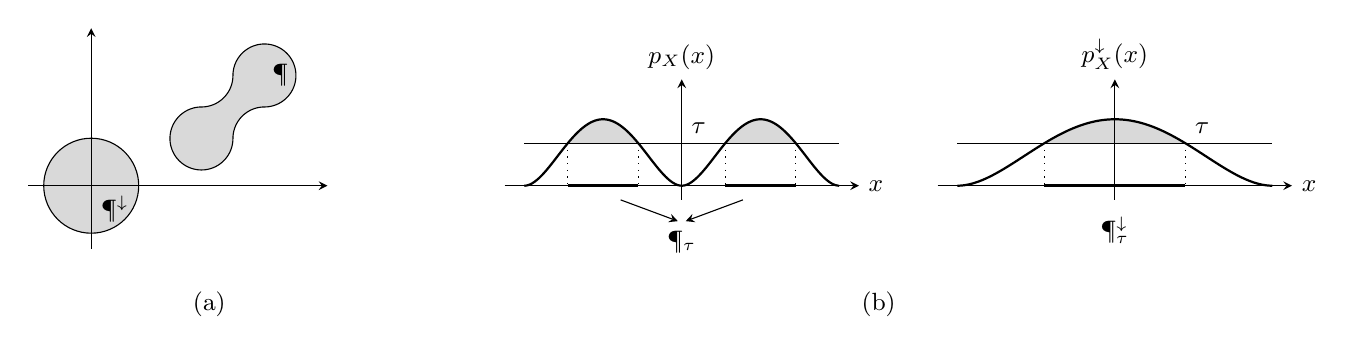
\begin{tikzpicture}
\shorthandoff{>}
%
\begin{scope}[scale=.4]
% Superficia 2*3 pi/4  + 2*2 - 2*pi/4 = 4+pi
\filldraw[draw=black,fill=gray!30]
   plot [domain=0:-270,samples=200] ({cos(\x)+3.5},{sin(\x)+1.5})
-- plot [domain=-90:0,samples=200] ({cos(\x)+3.5},{sin(\x)+3.5})
-- plot [domain=180:-90,samples=200] ({cos(\x)+5.5},{sin(\x)+3.5})
-- plot [domain=90:180,samples=200] ({cos(\x)+5.5},{sin(\x)+1.5})
-- cycle;
\draw (6,3.5) node {\small $\P$};
%
% superficia rearreglada
\filldraw[draw=black,fill=gray!30] (0,0) circle ({sqrt(1+4/pi)});
\draw (.75,-.75) node {\small $\P^\downarrow$};
%
% ejes
\draw[>=stealth,->] (-2,0)--(7.5,0);
\draw[>=stealth,->] (0,-2)--(0,5);
%
\end{scope}
%
%
%----------------------------------------
%
% p_X(x), P_tau...
\begin{scope}[xshift=7.5cm,yscale=1.8]
\pgfmathsetmacro{\t}{.3};
\pgfmathsetmacro{\xt}{sqrt(1-sqrt(32*\t/15))};
\pgfmathsetmacro{\dx}{5.5};% shift para p*(x)
\pgfmathdeclarefunction{studr}{1}{\pgfmathparse{(15/32)*((1-(#1)^2)^2)}}; %Student-r
%
% mezcla de Student-r 15/16 * (1-x^2)^2 (nu = 5) centrados en -1 y 1
% 15/32 (1-(x-a)^2)^2 > t iif (x-a)^2 < 1-sqrt(32*t/15)
% i.e. a-sqrt(1-sqrt(32*t/15)) < x < a+sqrt(1-sqrt(32*t/15))
\fill[domain=-1-\xt:-1+\xt,fill=gray!30] plot(\x,{studr(\x+1)}); % p(x) > tau, x < 0
\fill[domain=1-\xt:1+\xt,fill=gray!30] plot(\x,{studr(\x-1)}); % p(x) > tau, x > 0
\draw[thick,domain=-2:0,samples=100] plot(\x,{studr(\x+1)}); % p(x), x < 0
\draw[thick,domain=0:2,samples=100] plot(\x,{studr(\x-1)}); % p(x), x > 0
\draw (-2,\t)--(2,\t); \draw (0,\t) node[above right]{\small $\tau$}; % y = tau
%
% dominio P_tau
\draw[dotted] ({-1-\xt},{studr(\xt)})--({-1-\xt},0);
\draw[dotted] ({-1+\xt},{studr(\xt)})--({-1+\xt},0);
\draw[very thick] ({-1-\xt},0)--({-1+\xt},0);
\draw[>=stealth,->] ({-1+\xt/2},-.1)--(-.05,-.25);
%
\draw[dotted] ({1-\xt},{studr(\xt)})--({1-\xt},0);
\draw[dotted] ({1+\xt},{studr(\xt)})--({1+\xt},0);
\draw[very thick] ({1-\xt},0)--({1+\xt},0);
\draw[>=stealth,->] ({1-\xt/2},-.1)--(.05,-.25);
%
\draw (0,-.25) node[below]{\small $\P_\tau$};
%
% ejes
\draw[>=stealth,->] (-2.25,0)--(2.25,0) node[right]{\small $x$};
\draw[>=stealth,->] (0,-.1)--(0,.75) node[above]{\small $p_X(x)$};
%
%---------------------------
%
% 15/32 (1-(x-a)^2)^2 > t iif (x-a)^2 < 1-sqrt(32*t/15)
% i.e. a-sqrt(1-sqrt(32*t/15)) < x < a+sqrt(1-sqrt(32*t/15))
% Volumen 2*sqrt(1-sqrt(32*t/15))
% Por simetria, P_t* = [-2*sqrt(1-sqrt(32*t/15)) , 2*sqrt(1-sqrt(32*t/15))]
% da f*(x) = 15/32 (1-x^2/4)^2
\fill[domain=-2*\xt:2*\xt,fill=gray!30] plot({\x+\dx},{studr(.5*\x)}); % p*(x) > tau
\draw[thick,domain=-2:2,samples=200] plot({\x+\dx},{studr(.5*\x)});
\draw ({-2+\dx},\t)--({2+\dx},\t); \draw ({2*\xt+\dx},\t) node[above right]{\small $\tau$}; % y = tau
%
% dominio P_tau*
\draw[dotted] ({-2*\xt+\dx},{studr(\xt)})--({-2*\xt+\dx},0);
\draw[dotted] ({2*\xt+\dx},{studr(\xt)})--({2*\xt+\dx},0);
\draw[very thick] ({-2*\xt+\dx},0)--({2*\xt+\dx},0);
%
\draw (\dx,-.15) node[below]{\small $\P_\tau^\downarrow$};
%
% ejes
\draw[>=stealth,->] ({-2.25+\dx},0)--({2.25+\dx},0) node[right]{\small $x$};
\draw[>=stealth,->] (\dx,-.1)--(\dx,.75) node[above]{\small $p_X^\downarrow(x)$};
\end{scope}
%
\draw (1.5,-1.5) node{\small (a)};
\draw (10,-1.5) node{\small (b)};
\end{tikzpicture} \end{center}
%
\leyenda{(a):  Ilustraci\'on  del rearreglo  sim\'etrico  $\P^\downarrow$ de  un
  conjunto  $\P$,  siendo  la  bola   centrada  en  0  de  mismo  volumen.   (b)
  Construcci\'on  del  rearreglo  $p_X^\downarrow$:  dado un  $\tau$,  se  busca
  $\P_\tau$ y se deduce $P_\tau^\downarrow$; dado  un $x$, se busca el mayor $t$
  tal   que  $x  \in   P_t^\downarrow$,  este   $t$  m\'aximo   siendo  entonces
  $p_X^\downarrow(x)$; adem\'as, por construcci\'on, las superficies en gris son
  iguales.}
  %
\label{Fig:MP:ensemblerearreglado}
\end{figure}
% =  \B  \left( 0  , r_\P  \right)$ con  $\frac{2
%    \pi^{d/2} r_\P^d}{\Gamma(d/2)} = |\P|$.

A partir de esta definici\'on del rearreglo, se puede ahora extender la noci\'on
de mayorizaci\'on del caso discreto al caso continupo de la manera siguiente:
%
\begin{definicion}[Mayorizaci\'on en el contexto continuo]\label{Def:MP:MayorizacionC}
  Una densidad  de probabilidad $p$  es dicha mayorizada por  una distribuci\'on
  $q$ si:
  %
  \[
  p \prec  q \qquad \mbox{ssi}  \qquad \int_{\B(0,r)} p^\downarrow(x) \,  dx \le
  \int_{\B(0,r)} q^\downarrow(x) \, dx \quad \forall  \, r > 0, \quad \mbox{ y }
  \quad \int_{\Rset^d} p^\downarrow(x) \, dx = \int_{\Rset^d} q^\downarrow(x) \,
  dx,
  \]
  %
  donde \ $\B(0,r) = \{ x \in \Rset^d:  \: \|x\| \ge r \}$ \ es la bola centrada
  en \ $0$ \ y de rayo  \ $r$ \ (las \'ultimas integrales son obviamente iguales
  a 1).
\end{definicion}
%
\SZ{Equivalente de la curva de Lorentz???}


% ================================= Transformacion

\subseccion{Transformaci\'on de variables y vectores aleatorios}
\label{Ssec:MP:Transformacion}

En  esta  secci\'on nos  interesamos  al  effect de  una  variable  o un  vector
aleatorio. Por  ejemplo, en un juego con  dos dados, nos podemos  interesar a la
ley de la suma que dar\'ia el n\'umero de casilla de que debemos adelantar en un
juego de la oca.
%
\begin{teorema}[Transformaci\'on medible de un vector aleatorio]
  Sea  \  $X:  (\Omega,\A)  \mapsto  (\Rset^d ,  \B(\Rset^d))$  \  una  variable
  aleatoria,   y  \   $g:  (\Rset^d   ,  \B(\Rset^d))   \mapsto   (\Rset^{d'}  ,
  \B(\Rset^{d'}))$ \  una funci\'on  medible. Entonces,  \ $Y =  g(X)$ \  es una
  variable aleatoria  \ $(\Omega,\A)  \mapsto (\Rset^{d'} ,  \B(\Rset^{d'}))$. \
  Adem\'as, la medida im\'agen \ $P_Y$ \ es vinculada \ a \ $P_X$ \ por
  %
  \[
  \forall \, B \in \B(\Rset^{d'}), \quad P_Y(B) = P_X(g^{-1}(B)).
  \]
\end{teorema}
%
\begin{proof}
  Este resultado es obvio. $g$ siendo medible, para todo $B \in \B(\Rset^{d'})$,
  por definici\'on $g^{-1}(B) \in \B(\Rset^d)$.  Adem\'as, si $P_X$ es la medida
  (de  probabilidad) asociado  al  espacio de  salida  de $g$,  el resultado  es
  consecuencia  del   teorema  de  la   medida  im\'agen~\ref{Th:MP:MedidaImagen},
  pagina~\pageref{Th:MP:MedidaImagen}.
\end{proof}
%
\noindent (Ver ej.~\cite{JacPro03, AthLah06, Bog07:v2, Coh13}).


Es sencillo  probar de que  cualquier combinaci\'on de funciones  medibles queda
medible, cualquier  producto (adecuado) de  functiones medible queda  medible, y
que si $\{ f_k \}_{k=1}^{d'}$ son $(\B(\Rset^d),\B(\Rset))$-medible, entonces $f
=          (f_1         ,          \ldots         ,          f_{d'})$         es
$(\B(\Rset^d),\B(\Rset^{d'}))$-medible~\cite{AthLah06}.

% \SZ{No se  todav\'ia si ser\'a \'util  tratar del caso de l\'imite  de series de
%   funciones medibles.}


Mencionamos  de que si  $\X =  X(\Omega)$ es  discreto, entonces  $\Y =  g(\X) =
Y(\Omega)$ ser\'a discreto tambi\'en, y:
%
\begin{teorema}[Funci\'on de masa por transformaci\'on medible]
  Sean   $X$,   vector  aleatorio   $d$-dimensional   discreto,  $g:(\Rset^d   ,
  \B(\Rset^d)) \mapsto (\Rset^{d'} , \B(\Rset^{d'}))$ una funci\'on medible, e \
  $Y =  g(X)$ necesariamente discreto  $d'$-dimensional sobre $\Y =  g(\X)$.  La
  distribuci\'on de $Y$ es relacionada a la de $X$ por la relaci\'on
  %
  \[
  \forall \, y \in \Y, \quad p_Y(y) = \sum_{x \in g^{-1}(y)} p_X(x).
  \]
\end{teorema}
%
\begin{proof}
El resultado es inmediato.
\end{proof}
%
\noindent En particular,  si $g$ es inyectiva (necesariamente  biyectiva de $\X$
en $\Y$),  el vector  de probabilidad queda  invariante, $p_Y =  p_X$; solamente
cambian los estados.

Es  importante mencionar de  que con  $\Y$ discreto,  $\X$ no  es necesariamente
discreto~\cite{AthLah06}. Por ejemplo, $Y = \un_{X>0}$  es tal que $\Y = \{ 0 \,
; \, 1 \}$ a pesar de que $\X$ puede ser no discreto.

Tratar de las variables aleatorias  continuas resuelta mas delicado. Vimos en el
ejemplo   precediente  de   que  el   caracter  continuo   puede   perderse  por
transformaci\'on. De la misma manera, en un ejemplo de la secci\'on precediente,
vimos  que  $Y =  X_1  \un_{X_2>0}$ con  $X_i$  independientes  uniformes es  ni
continua,  ni  discreta.  En  el  enfoque  de  variables  continuas,  una  clase
importante  de funciones  en la  cual  no vamos  a interesar  son las  funciones
continuas (y diferenciables):
%
\begin{lema}[Continuidad y caracter medible]
  Sea   $g:   \Rset^d   \mapsto   \Rset^{d'}$   continua.   Entonces,   $g$   es
  $(\B(\Rset^d),\B(\Rset^{d'}))$-medible.
\end{lema}
%
\begin{proof}
  Por continuidad,  la pre-im\'agen de  un abierto de  $\Rset^{d'}$ por $g$  es un
  abierto  de $\Rset^d$  y entonces  es en  $\B(\Rset^d)$. La  prueba  se cierra
  recordandose  de  la   definici\'on  de  $\B(\Rset^{d'})$,  $\sigma$-\'algebra
  generada por los abiertos de $\Rset^{d'}$.
\end{proof}

En lo  que sigue, nos interesamos  m\'as especialmente al caso  de funciones $g:
(\Rset^d ,  \B(\Rset^d)) \mapsto (\Rset^d ,  \B(\Rset^d))$.  De hecho,  si $d' <
d$,   es    sencillo   llegar   al   caso    considerado   a\~nandiendo   $d-d'$
transformaciones. Por ejemplo, con $d = 2$  si nos interesamos a $X_1 + X_2$, se
puede considerar $\begin{bmatrix} X_1 + X_2 & X_2 - X_1\end{bmatrix}^t$ y llegar
a la variable de  inter\'es por calculo de marginal. Si $d'  > d$ la situaci\'on
es  m\'as  delicada,  $g(Y)$  viviendo  sobre una  variedad  $d$-dimensional  de
$\Rset^{d'}$.

En  el caso  de vectores  aleatorios continuos  $X$ admitiendo  una  densidad de
probabilidad,  una pregunta  natural  es entonces  de  saber si  se conserva  la
continuidad y la existencia de una densidad, as\'i que su forma. La respuesta es
dada por el teorema siguiente~\cite{Bre88, JacPro03, AthLah06, Coh13, HogMck13}:
%
\begin{teorema}[Densidad de probabilidad por transformaci\'on continua inyectiva diferenciable]
  Sean $X$, vector aleatorio  $d$-dimensional continuo y admitiendo una densidad
  de probabilidad  $p_X$, \ $g:\Rset^d  \mapsto \Rset^d$ una  funci\'on continua
  inyectiva y diferenciable tal que
  %  ~\footnote{\modif{De  hecho,  se   puede  extender  el  resultado  para  un
  %      determinente del  Jacobiano cancelandose  en  un conjunto  de punto  de
  %     medida  de Lebesgue nula y en  los $y$ donde se  cancela el determinente
  %       del  Jacobiano,  la   densidad  va   a  ser   divergente  (divergencia
  %     integrable).}}
 $\left| \Jac_g \right| > 0$,
  %
 donde $\Jac_g$ denota la  matriz de componentes \ $\frac{\partial g_i}{\partial
   x_j}$, \ matriz Jacobiana de  la transformaci\'on \ $g \equiv \begin{bmatrix}
   g_1(x_1 , \ldots , x_d) & \cdots & g_d(x_1 , \ldots , x_d) \end{bmatrix}^t$ \
 y \ $|\cdot|$ representa el valor absoluto del determinante de la matriz. Sea \
 $Y = g(X)$.   Entonces $Y$ es continua admitiendo  una densidad de probabilidad
 $p_Y$ de soporte $\Y = g(\X) = Y(\Omega)$ tal que
  %
  \[
  \forall \,  y \in  \Y, \quad p_Y(y)  = p_X(g^{-1}(y))  \left| \Jac_{g^{-1}}(y)
  \right|.
  \]
\end{teorema}
%
\begin{proof}
Por definici\'on, $X$ admitiendo una densidad y $g$ siendo medible,
%
\[
\forall \, B  \in \B(\Rset^d), \quad P_Y(B) =  P_X(g^{-1}(B)) = \int_{g^{-1}(B) \cap \X}
p_X(x) \, dx.
\]
%
Por cambio de variable $x =  g^{-1}(y)$ ($g$ siendo inyectiva, el antecedante es
\'unico por definic\'on) y notando de que $g\left( g^{-1}(B) \cap \X \right) = B
\cap \Y$,
%
\[
\forall \, B \in \B(\Rset^d), \quad  P_Y(B) = \int_{B \cap \Y} p_X(g^{-1}(y)) \,
\left| \Jac_{g^{-1}}(y) \right| \, dy
\]
%
lo que cierra la prueba~\footnote{La aparici\'on de la Jacobiana viene del mismo
  enfoque que  el cambio de variables  en la integraci\'on de  Rieman. De hecho,
  como lo hemos visto, $\mu_L(B) = |B|$ es el volumen y de la definici\'on mismo
  del  determinente, para  cualquier matriz  cuadrada  el volumen  se escribe  \
  $\mu_L(M  B) =  |M B|  = |M|  |B|  = |M|  \mu_L(B)$ donde  la misma  escritura
  $|\cdot|$ representa  el valor absoluto  del determinente de una  matriz. Esta
  notaci\'on se justifica  precisamente por su significaci\'on de  volumen, y el
  resultado  es  inmediato  para $g(x)  =  M  x$.  La  forma general,  para  una
  transformaci\'on m\'as  general a  partir de un  desarollo de Taylor  al orden
  1~\cite{AthLah06, Coh13}.}.
\end{proof}

El caso escalar puede ser visto como caso particular, dando:
%
\begin{corolario}
  Sean  $X$,   variable  aleatoria  continua   y  admitiendo  una   densidad  de
  probabilidad $p_X$, $g:\Rset \mapsto  \Rset$ una funci\'on continua, inyectiva
  y  diferenciable e  \ $Y  = g(X)$.   Entonces $Y$  es continua  admitiendo una
  densidad de probabilidad $p_Y$ tal que
  %
  \[
  \forall  \,   y  \in  \Y,   \quad  p_Y(y)  =  p_X(g^{-1}(y))   \left|  \frac{d
      g^{-1}(y)}{dy} \right|.
  \]
\end{corolario}
%
\noindent  De hecho,  se puede  ver estos  resultados esquematicamente  como una
``conservaci\'on'' de  probabilidad, $p_X(x)  dx = p_Y(y)  dy$, el  volumen $dy$
siendo   relacionado  al  $dx$   a  traves   de  la   Jacobiana  (ver   nota  de
pie~\ref{Foot:SZ:Jacobiana}).

Una  forma  alternativa  de derivar  este  corrolario  consiste  a salir  de  la
funci\'on   de   repartici\'on,   notando   de   que   $g$   es   necesariamente
mon\'otona~\footnote{Fijense de que $P(X \ge x) = 1 -  P(X < x) = 1 - P(X \le x) +
  P(X =  x)$, pero $X$ siendo  continua, $ P(X =  x) = 0$.}: si  $y \not\in \Y$,
necesariamente $p_Y = 0$ ($F_Y(y) = 1$ \ si \ $y > \sup \Y$ \ y \ $F_Y(y) = 0$ \
si \ $y < \inf \Y$) \ y para cualquier \ $y \in \Y$,
%
\[
F_Y(y) = P(Y \le y) = P(g(X) \le y) =
\left\{\begin{array}{lll}
P(X \le g^{-1}(y)) = F_X(g^{-1}(y)) & \mbox{si} & g \quad \mbox{es creciente}\\[2.5mm]
%
P(X \ge g^{-1}(y)) = 1 - F_X(g^{-1}(y)) & \mbox{si} & g \quad \mbox{es decreciente}
\end{array}\right..
\]
%
El  resultado  se  obtiene  calculando  las  derivadas  del  primer  y  \'ultimo
t\'erminos respecto de la variable transformada $y$.

Si $g$ no es inyectiva, $g^{-1}$  es multivaluada o multiforme. En este caso, se
puede todav\'ia  tratar el problema, particionando $\Rset^d$  en conjuntos donde
$g$ es inyectiva, dando
%
\begin{teorema}
  Sean $X$, vector aleatorio  $d$-dimensional continuo y admitiendo una densidad
  de  probabilidad   $p_X$,  $g:(\Rset^d  ,  \B(\Rset^d))   \mapsto  (\Rset^d  ,
  \B(\Rset^d))$  una  funci\'on continua  y  diferenciable.  Denotamos  $\left\{
    \X_{[k]} \right\}_{k=0}^m$ la partici\'on  de $\X$ tal que $\left| \Jac_g(y)
  \right| = 0$ sobre  $\X_{[0]}$ y para todos $k \ge 1$,  \ $g: \X_{[k]} \mapsto
  \Y$ \ sea inyectiva y tal que \ $\left| \Jac_g(y) \right| > 0$. \ Suponemos de
  que  $\X_{[0]}$ sea  de medida  de Lebesgue  nula, notamos  \ $g_k^{-1}$  \ la
  funci\'on inversa de  \ $g$ \ sobre \ $g(\X_{[k]})$ \  (rama $k$-\'esima de la
  funci\'on multivaluada $g^{-1}$), \  $\Jac_{g_k^{-1}}$ \ su matriz Jacobiana y
  \ $I(y) = \{ k, \: y \in g(\X_{[k]}) \}$ \ los indices tales que \ $y$ \ tiene
  un      inverso     por      $g_k$.      Esto      es      ilustrado     figura
  Fig.~\ref{Fig:MP:TransformacionVA}  para $d  = 1$.   Entonces $Y$  es continua
  admitiendo una densidad de probabilidad $p_Y$ tal que
  %
  \[
  \forall  \, y  \in \Y,  \quad p_Y(y)  = \sum_{k  \in  I(y)} p_X(g_k^{-1}(y))
  \left| \Jac_{g_k^{-1}}(y) \right|.
  \]
  %
  En el caso escalar $d = 1$ esto se formula
  %
  \[
  \forall \, y \in \Y, \quad  p_Y(y) = \sum_{k \in I(y)} p_X(g_k^{-1}(y)) \left|
    \frac{d g_k^{-1}(y)}{dy} \right|.
  \]
\end{teorema}
%
\begin{proof}
  Sufice escribir  \ $B  = \bigcup_{k =  0}^m \left(  B \cap g(\X_k)  \right)$ \
  uni\'on de borelianos disjuntos, notar  de que por consecuencia \ $g^{-1}(B) =
  \bigcup_{k =0}^m g^{-1}\left( B \cap  g(\X_k) \right)$ \ uni\'on de borelianos
  disjuntos \  y \  por linearidad escribir  la integraci\'on  sobre $g^{-1}(B)$
  como la  suma de  integrales sobre $g^{-1}\left(  B \cap g(\X_k)  \right)$. Se
  cierra la  prueba notando de  que \ $g^{-1}\left(  B \cap g(\X_0)  \right)$ es
  necesario  de medida de  Lebesgue nula,  siendo la  integral nula  y de  que \
  $g^{-1}\left( B \cap g(\X_k) \right) = g_k^{-1}\left( B \cap g(\X_k) \right)$.
\end{proof}
%

\begin{ejemplo}[Ejemplo de transformaci\'on no biyectiva]
  Sea $X$ definido sobre  \ $\X = \Rset$ \ y la  transformaci\'on de variables \
  $Y = X^2$.   Se tiene \ $y  = g(x) = x^2$, continua  diferenciable de derivada
  nula  sobre \  $\X_{[0]} =  \{ 0  \}$, de  medida nula,  cuyas inversas  son \
  $g_1^{-1}(y) = \sqrt{y}$ \ sobre \ $\X_{[1]} = \Rset_-^*$ \ y \ $g_2^{-1}(y) =
  -   \sqrt{y}$  sobre   \   $\X_{[2]}   =  \Rset_+^*$;   luego   \  $p_Y(y)   =
  \frac{p_X(\sqrt{y})  +   p_X(-\sqrt{y})}{2  \sqrt{y}}$,   \  sobre  \   $\Y  =
  \Rset_+^*$.
\end{ejemplo}

De nuevo, en el caso escalar, se puede salir de la funci\'on de repartici\'on
%
\[
F_Y(y) =  P(Y \le y) = P(  g(X) \le y )  = \sum_{k=1}^m P\left( X  \in \X_{[k]} \cap
  g_k^{-1}(-\infty \, ; \, y] \right)
\]
%
($\X_{[0]}$  siendo  de medida  nula,  sobre  este  dominio la  probabilidad  es
cero). Sea $\Y_{[k]} = g_k(\X_{[k]})$. Ahora, si $y \not\in I(y)$,
%
\[
P\left(   X   \in  \X_k   \cap   g_k^{-1}(-\infty  \,   ;   \,   y]  \right)   =
\left\{\begin{array}{lll}
%
P(X \in \X_{[k]}) & \mbox{si} & y > \sup \Y_{[k]}\\[2.5mm]
%
0 & \mbox{si} & y < \inf \Y_{[k]}\\[2.5mm]
\end{array}\right.
\]
%
dando una derivada nula. Si $y \in I(y)$,
%
\[
P\left(   X   \in  \X_k   \cap   g_k^{-1}(-\infty  \,   ;   \,   y]  \right)   =
\left\{\begin{array}{lll}
%
F_X(g_k^{-1}(y)) - F_X(\inf \Y_{[k]}) & \mbox{si} & g_k \quad \mbox{es creciente}\\[2.5mm]
%
F_X(\sup \Y_{[k]}) - F_X(g_k^{-1}(y))  & \mbox{si} & g_k \quad \mbox{es decreciente}
\end{array}\right..
\]
%
El  resultado  sigue  diferenciando  este  resultado. Esto  es  ilustrado  figura
Fig.~\ref{Fig:MP:TransformacionVA}.

\begin{figure}[h!]
\begin{center} 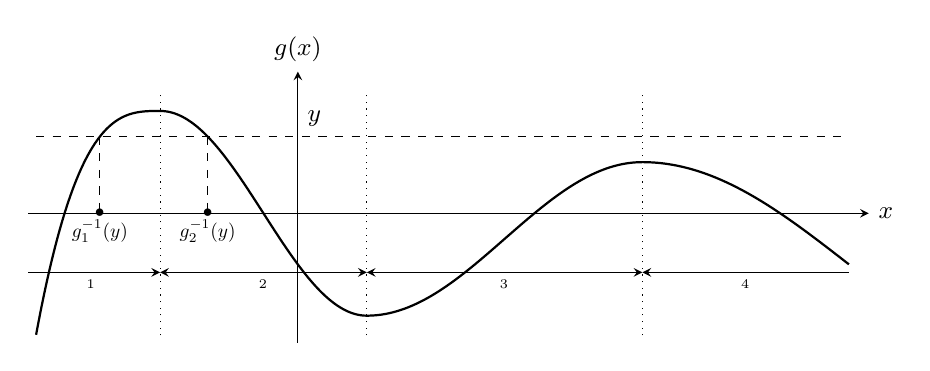
\begin{tikzpicture}%[scale=.9]
\shorthandoff{>}
%
\pgfmathsetmacro{\sx}{1.75};% x-scaling
%
% transformacion g' = 0 medida nula
\begin{scope}
%
\pgfmathsetmacro{\sy}{1.3};% y-scaling 
%
\draw[>=stealth,->] ({-1.9*\sx-.1},0)--({\sx*4+.25},0) node[right]{\small $x$};
\draw[>=stealth,->] (0,{\sy*(-3*.9^3+1)-.1})--(0,{\sy+.5}) node[above]{\small $g(x)$};
%
\draw[thick]
plot[domain=-1.9:-1,samples=100] ({\sx*\x},{\sy*(3*(\x+1)^3+1)})
-- plot[domain=-1:.5,samples=100] ({\sx*\x},{\sy*cos(120*(\x+1))})
-- plot[domain=.5:2.5,samples=100] ({\sx*\x},{\sy*(.75*sin(90*(\x-1.5))-.25)})
-- plot[domain=2.5:4,samples=100] ({\sx*\x},{\sy*(cos(60*(\x-2.5))-.5)})
;
%
\draw[dashed] ({-1.9*\sx},{.75*\sy})--({4*\sx},{.75*\sy});
\draw (0,{.75*\sy}) node[above right]{\small $y$};
%
\draw[dashed] ({-\sx*(1+(.25/3)^(1/3))},{.75*\sy})--({-\sx*(1+(.25/3)^(1/3))},0)
node[scale=.7]{$\bullet$} node[below,scale=.7]{$g_1^{-1}(y)$};
%
\draw[dashed] ({\sx*(acos(.75)/120-1)},{.75*\sy})--({\sx*(acos(.75)/120-1)},0)
node[scale=.7]{$\bullet$} node[below,scale=.7]{$g_2^{-1}(y)$};
%
%
\draw[dotted] ({-\sx},{-\sy-.25})--({-\sx},{\sy+.25});
\draw[>=stealth,->] ({-\sx*1.9-.1},-.75)--({-\sx},-.75);
\draw ({-1.5*\sx},-.75) node[below,scale=.8]{\small $\X_1$};
%
\draw[dotted] ({.5*\sx},{-\sy-.25})--({.5*\sx},{\sy+.25});
\draw[>=stealth,<->] ({-\sx},-.75)--({.5*\sx},-.75);
\draw ({-.25*\sx},-.75) node[below,scale=.8]{\small $\X_2$};
%
\draw[dotted] ({2.5*\sx},{-\sy-.25})--({2.5*\sx},{\sy+.25});
\draw[>=stealth,<->] ({.5*\sx},-.75)--({2.5*\sx},-.75);
\draw ({1.5*\sx},-.75) node[below,scale=.8]{\small $\X_3$};
%
\draw[>=stealth,<-] ({2.5*\sx},-.75)--({4*\sx},-.75);
\draw ({3.25*\sx},-.75) node[below,scale=.8]{\small $\X_4$};
\end{scope}
%
%
% % reparticion
% \begin{scope}[xshift=8.5cm]
% %
% \pgfmathsetmacro{\sy}{2};% y-scaling 
% %
% \draw[>=stealth,->] (-.6,0)--({\sx*4+.25},0) node[right]{\small $x$};
% \draw[>=stealth,->] (0,-.25)--(0,{\sy+.5}) node[above]{\small $F_X$};
% %
% \draw[thick] (-.5,0)--(0,0)--(\sx,{\sy/2})--({2*\sx},{\sy/2})
% -- plot[domain=2:3,samples=100] ({\sx*\x},{\sy*(1+(\x-2)^(3/2))/2})
% -- ({\sx*4},\sy);
% %
% \draw (\sx,0)--(\sx,-.1) node[below,scale=.9]{\small $1$};
% \draw ({2*\sx},0)--({2*\sx},-.1) node[below,scale=.9]{\small $2$};
% \draw ({3*\sx},0)--({3*\sx},-.1) node[below,scale=.9]{\small $3$};
% \draw (\sx,0)--(\sx,-.1) node[below,scale=.9]{\small $1$};
% %
% \draw (0,{\sy/2})--(-.1,{\sy/2}) node[left,scale=.7]{\small $1/2$};
% \draw (0,\sy)--(-.1,\sy) node[left,scale=.7]{\small $1$};
% %
% \draw ({\sx*2.25},-1) node{\small (b)};
% \end{scope}
%
\end{tikzpicture} \end{center}
%
\leyenda{(a): Ilustraci\'on  de una transformaci\'on  $g$ no inyectiva,  tal que
  $\X_{[0]} = \{ x, \: g'(x) = 0 \}$, representado por las lineas punteadas ($x$
  correspondiente), es de medida de  Lebesgue nula.  Los $\X_{[k]}$ son descrito
  debajo de cada dominio.  La linea discontinua  da un nivel $y$ y los puntos en
  el eje $x$ representan $g_k^{-1}(y), \: k \in I(y)$; en el ejemplo, $I(y) = \{
  1  \,  ;  \,  2 \}$  \  y,  suponiendo  de  que  $\X  = \Rset$,  \  $F_Y(y)  =
  F_X(g_1^{-1}(y)) + 1-F_X(g_2^{-1}(y))$.}
\label{Fig:MP:TransformacionVA}
\end{figure}

Una  tercera alternativa,  a pesar  que sea  delicado, es  de apoyarse  sobre la
teoria de las  distribuciones y expresar como \  $\displaystyle p_Y(y) = \int_\X
p_X(x) \,  \delta(y-g(x)) \, dx$,  donde se usa  la expansi\'on de  la funci\'on
delta  en  t\'erminos de  sus  ceros:  \  $\delta(y-g(x)\,)= \sum_{k  \in  I(y)}
\frac{1}{\left|      g_k'\left(      g_k^{-1}      (y)     \right)      \right|}
\delta(x-g_k^{-1}(y))$~\cite{ManWol95}.

Es  importante  notar  de  que  la  condici\'on $\X_{[0]}$  de  medida  nula  es
importante. El el caso contrario, $Y$ no  queda continua como se lo puede ver en
el ejemplo siguiente.
%
\begin{ejemplo}[Transformaci\'on con $\mu_L\left( \X_{[0]} \right) \ne 0$]
  Sea \ $X$ \  uniforme sobre \ $\X = ( 3 \,  ; \, 3)$ \ y \ $Y  = g(X)$ \ con \
  $g(x) = \left( 1 + \cos\left( (|x|-1) \frac{\pi}{2} \right) \right) \un_{(1 \,
    ; \,  3)}(|x|) + 2 \un_{[0  \, ; 1]}(|x|)$.  Esta  funci\'on es representado
  figura Fig.~\ref{Fig:MP:TransformacionVANoContinua}-(a).   Claramente, \ $g$ \
  es continua y  diferenciable sobre $\X$, pero con  \ $\X_{[0]} = [ -1  \, ; \,
  1]$ que no es de medida nula.  Saliendo de $F_Y(y) = P(g(X) \le y)$ se calcula
  sencillamente  $F_Y(y) =  \frac23 \left(  1 -  \frac1\pi  \arccos(y-1) \right)
  \un_{[0  \, ;  \,  2)} +  \un_{[ 2  \,  ; \,  +\infty)}(y)$, ilustrada  figura
  Fig.~\ref{Fig:MP:TransformacionVANoContinua}-(b).   Claramente  \  $F_Y$ \  es
  discontinua en \ $y = 2$: \ $Y$ \ no es continua.
  %
  \begin{figure}[h!]
  \begin{center} \begin{tikzpicture}%[scale=.9]
\shorthandoff{>}
%
\pgfmathsetmacro{\r}{.05};% radius arc non continuity F_X y/o p_X
%
% transformacion g' = 0 medida no nula
\begin{scope}
%
\draw[>=stealth,->] (-3.6,0)--(3.75,0) node[right]{\small $x$};
\draw[>=stealth,->] (0,-.25)--(0,2.5) node[above]{\small $g(x)$};
%
\draw[thick]
(-3.4,0)--(-3,0)--
plot[domain=-3:-1,samples=100] (\x,{1+cos(90*(1+\x))})--
(1,2)--
plot[domain=1:3,samples=100] (\x,{1+cos(90*(1-\x))})--
(3.5,0);
%
\draw (-3,0)--(-3,-.1) node[below,scale=.8]{\small $-3$};
\draw (-2,0)--(-2,-.1) node[below,scale=.8]{\small $-2$};
\draw (-1,0)--(-1,-.1) node[below,scale=.8]{\small $-1$};
\draw (1,0)--(1,-.1) node[below,scale=.8]{\small $1$};
\draw (2,0)--(2,-.1) node[below,scale=.8]{\small $2$};
\draw (3,0)--(3,-.1) node[below,scale=.8]{\small $3$};
%
\draw (0,1)--(-.1,1) node[left,scale=.8]{\small $1$};
\draw (-.1,2) node[above left,scale=.8]{\small $2$};
%
\draw[>=stealth,<->] (-3,-.5)--(-1,-.5); \draw (-2,-.5) node[below,scale=.9]{\small $\X_{[1]}$};
\draw[>=stealth,<->] (1,-.5)--(3,-.5); \draw (2,-.5) node[below,scale=.9]{\small $\X_{[2]}$};
\draw[>=stealth,<->] (-1,-.5)--(1,-.5); \draw (0,-.5) node[below,scale=.9]{\small $\X_{[0]}$};
%
\draw(0,-1.5) node{\small (a)};
\end{scope}
%
%
% reparticion
\begin{scope}[xshift=7cm]
%
\pgfmathsetmacro{\sx}{1.5};
\pgfmathsetmacro{\sy}{2};% y-scaling 
%
\draw[>=stealth,->] (-.6,0)--({3*\sx+.5},0) node[right]{\small $y$};
\draw[>=stealth,->] (0,-.25)--(0,{\sy+.25}) node[above]{\small $F_Y$};
%
\draw[thick] (-.5,0)--(0,0)--
plot[domain=0:2,samples=250] ({\sx*\x},{\sy*2*(1-acos(\x-1)/180)/3});
%
\draw ({2*\sx+\r},{2*\sy/3+\r}) arc (90:260:\r);
%--
\draw[dotted] ({2*\sx},{2*\sy/3})--({2*\sx},\sy);
\draw[thick] ({2*\sx},\sy) node[scale=.7]{$\bullet$}--({3*\sx},\sy);
%
\draw ({\sx},0)--({\sx},-.1) node[below,scale=.8]{\small $1$};
\draw ({2*\sx},0)--({2*\sx},-.1) node[below,scale=.8]{\small $2$};
\draw ({3*\sx},0)--({3*\sx},-.1) node[below,scale=.8]{\small $3$};
%
\draw (0,{2*\sy/3})--(-.1,{2*\sy/3}) node[left,scale=.7]{\small $2/3$};
\draw (0,\sy)--(-.1,\sy) node[left,scale=.7]{\small $1$};
%
\draw({1.75*\sx},-1.5) node{\small (b)};
\end{scope}
%
\end{tikzpicture} \end{center}
  %
  \leyenda{En (a) se dibuja $g(x)  = \left( 1 + \cos\left( (1-|x|) \frac{\pi}{2}
      \right)   \right)  \un_{(1   \,  ;   \,  3)}(|x|)   +  2   \un_{[0   \,  ;
      1]}(|x|)$. Suponiendo de que $\X = (-3 \, ; \, 3)$, claramente $\X_{[0]} =
    [ -1 \, ; \, 1]$ no es de medida nula, dando para $X$ uniforme sobre $\X$ la
    variable $Y = g(X)$ no  continua de funci\'on de repartici\'on representenda
    en (b).  }
  \label{Fig:MP:TransformacionVANoContinua}
  \end{figure}
\end{ejemplo}

Un ejemplo de  cambio de transformaci\'on puede sevir a  calcular la densidad de
probabilidad de una suma:
%
\begin{ejemplo}[Distribuci\'on de la suma de vectores aleatorios]\label{Ej:MP:Suma}
  Sean \  $X$ \ e  \ $Y$ \  dos vectores aleatorios conjuntamente  continuos, de
  densidad de  probabilidad conjunta $p_{X,Y}$,  y sea el  vector \[V = X  + Y.\]
  Queremos calcular la a partir de la densidad de probabilidad de $V$.  Por esto,
  se puede considerar la transformaci\'on biyectiva
  %
  \[
  g: (x,y) \mapsto (u,v) = (x,x+y).
  \]
  %
  Entonces
  %
  \[
  g^{-1}(u,v) = (u,v-u)
  \]
  %
  y la matriz Jacobiana es
  %
  \[
  J_{g^{-1}} = \begin{bmatrix} I & -I \\ 0 & I \end{bmatrix}
  \]
  %
  donde $I$ es la matriz identidad $d$-dimensional y $0$ la matriz nula de misma
  dimension. Claramente\ $\left| J_{g^{-1}} \right| = 1$ \ as\'i que
  %
  \[
  p_{U,V}(u,v) = p_{X,Y}(u,v-u)
  \]
  %
  como lo pudimos intuir. Adem\'as, por marginalizaci\'on, inmediatamente
  %
  \[
  p_V(v) = \int_{\Rset^d} p_{X,Y}(u,v-u) \, du.
  \]
  %
  Si \ $X$ \ e \ $Y$  \ son independientes, \ $p_{U,V}(u,v) = p_X(u) p_V(v-u)$ \
  y la f\'ormula integral se escribe
  %
  \[
  p_V(v) = \int_{\Rset^d} p_X(u) p_Y(v-u) \, du = \int_{\Rset^d} p_Y(u) p_X(v-u)
  \, du
  \]
  %
  (por  cambio  de variable  en  la  secunda  expresi\'on).  Esta  f\'ormula  es
  conocida    como     {\it    producto    de     convoluci\'on}    entre    las
  funciones~\footnote{Este  producto  no  impone   de  que  las  funciones  sean
    densidades de  probabilidad.  Una condici\'on suficiente para  que existe es
    que     las     funciones     sean     $L^1$     (ver     desigualdad     de
    Cauchy-Bunyakovsky-Schwarz).} $p_X$ y $p_Y$.
\end{ejemplo}


%|q(y^1,\ldots,y^d)\ dy^1\cdots dy^d| = |p(x^1,\ldots,x^d) \ dx^1\cdots dx^d| .

%% Ejercicio: Estudiar el caso multivaluado / Resolver un ej. 

\

\aver{\SZ{No toque todav\'ia. Se puede hacerlo con vectores. Caso circular\ldots}

\hfill

Una  \emph{variable  aleatoria  compleja}   $Z=X+i  Y$  puede  interpretarse  en
t\'erminos de las  dos variables aleatorias reales $X$ e $Y$.  La pdf asociada \
$P(z)=p(x,y)$ est\'a dada por la  funci\'on densidad de probabilidad conjunta de
las variables reales. La condici\'on de normalizaci\'on se escribe
%
$$
\int P(z) \, d^2 z = 1
$$
%
donde $d^2 z=dx\,dy$.
}


% ================================= Vector discreto

\subseccion{Leyes condicionales}
\label{Ssec:MP:LeyesCondicionales}

Tratando de un par de vectores aleatorios  \ $X$ \ e \ $Y$, una pregunta natural
puede ser de caracterizar el vector  $Y$ si ``observamos $X = x$''. En palabras,
la pregunta es de describir la ley de $Y$ ``sabiendo de que $X = x$''. En lo que
sigue, para  fijar las notaciones, consideramos  $(X,Y): ( \Omega  , \A) \mapsto
(\Rset^{d_X} \! \times \Rset^{d_Y} \, , \, \B(\Rset^{d_X} \! \times \Rset^{d_Y})
)$ tal que $X$ sea $d_X$-dimensional e $Y$ sea $d_Y$-dimensional (incluyendo los
casos escalares).


% ---------- Caso discreto

\paragraph{Caso $\boldsymbol{X}$ discreto:}
Un caso  sencillo a estudiar  es cuando $\X  = X(\Omega)$ es discreto.   En este
caso, para  cualquier $x  \in \X$, tenemos  $P_X(x) = P(X  = x)  \ne 0$ y  de la
definici\'on de  la probabilidad condicional Def.~\ref{Def:MP:ProbaCondicional},
$P(Y \in A | X = x) = \frac{P(Y \in A \cap X = x)}{P(X=x)}$ define una medida de
probabilidad que llamamos medida de probabilidad condicional y que notaremos
%
\[
P_{Y|X=x}(A) = P(Y \in A | X = x).
\]
%
Siendo una medida de probabilidad, se puede referirse a la subsecci\'on anterior
para  definir  una  funci\'on   de  repartici\'on  tomando  $\displaystyle  A  =
\prod_{i=1}^d (-\infty \, ; \,  y_i]$, caracterisando completamento la medida de
probabilidad:
%
\begin{definicion}[Funci\'on de repartici\'on condicional ($X$ discreto)]
  Por definici\'on, la funci\'on de repartici\'on condicional es,
  %
  \[
  \forall \:  x \in  \X, \: y  \in \Y, \quad  F_{Y|X=x}(y) =  P( \left. Y  \le y
  \right|  X =  x  ) =  \frac{P\left(Y  \le y  \cap X  =  x \right)}{P\left(X  =
      x\right)}.
  \]
\end{definicion}

Ahora, cuando $Y$ est discreta tambi\'en,  se puede definir la funci\'on de masa
discreta  de probabilidad,  y  si $Y$  es  continua admitiendo  una densidad  de
probabilidad, se puede definir una densidad de probabilidad condicional:
%
\begin{definicion}[Funci\'on de masa o densidad de probabilidad condicional ($X$
  discreto)]
  Por  definici\'on,  cuando  $\Y$  est   discreto,  la  funci\'on  de  masa  de
  probabilidad condicional es,
  %
  \[
  \forall \:  x \in  \X, \: y  \in \Y, \quad  p_{Y|X=x}(y) =  P( \left. Y  = y
  \right|  X =  x  ) =  \frac{P\left(Y  = y  \cap X  =  x \right)}{P\left(X  =
      x\right)}.
  \]
  %
  Si $Y$ es continua, es sencillo  ver de que $P_{Y|X=x} \ll P_Y$, i.e., $P_Y(B)
  = 0  \: \Rightarrow  \: P_{Y|X=x}(B) =  0$.  Si  $Y$ adminte una  densidad con
  respecto a la medida de Lebesgue,  $P_Y \ll \mu_L$ medida de Lebesgue, es claro
  de    que   tambi\'en   $P_{Y|X=x}    \ll   \mu_L$,    y   por    teorema   de
  Radon-Nikod\'ym~\ref{Th:MP:RadonNikodym}, admite  una densidad de probabilidad
  (con respecto a la medida de Lebesgue) que denotaremos $p_{Y|X=x}$,
  %
  \[
  \forall \: B, \quad P_{Y|X=x}(B) = \int_B p_{Y|X=x}(y) \, dy.
  \]
  %
  Saliendo de la funci\'on de repartici\'on, obtenemos
  %
  \[
  p_{Y|X=x}(y) = \frac{\partial^{d_Y} F_{Y|X=x}(y)}{\partial y_1 \ldots \partial
    y_{d_Y}}.
  \]
\end{definicion}


% ---------- Caso continuo

\paragraph{Caso $\boldsymbol{X}$ continuo admitiendo una densidad:}
Cuando  $X$ es  continuo, el  problema aparece  m\'as subtile  porque  $P(X=x) =
0$. Entonces, no  se puede usar la definici\'on  de la probabilidad condicional,
el evento $(X=x)$ siendo de probabilidad cero.  Sin embargo, se puede seguir los
pasos  de  R\'enyi~\cite[Cap.~5]{Ren} por  ejemplo  para  resolver el  problema,
llegando a un resultado tan intuitivo que en el caso discreto.

Por esto, sea $B \in \B(\Rset^{d_Y})$ y definimos la medida $\nu_B(A) = P(X \in A
\cap Y  \in B)$ sobre  $(\Rset^{d_Y},\B(\Rset^{d_Y}))$.  Es sencillo ver  de que
$B$ siendo dado, $\nu_B$ define una medida de probabilidad. Adem\'as, $\nu_B \ll
P_X$, i.e., $P_X(A) = P(X \in A) = 0  \: \Rightarrow \: 0 = P(X \in A \cap Y \in
B)  =  \nu_B(A)$.    Por  teorema  de  Radon-Nikod\'ym~\ref{Th:MP:RadonNikodym},
$\nu_B$ admite una densidad $g_B$ con respecto a $P_X$,
%
\[
\forall \: A, \quad P\left( (X \in A)  \cap (Y \in B) \right) = \int_A g_B(x) \,
dP_X(x).
\]
%
Claramente \ $g_B \ge 0$,  \ y de \ $P(X \in A) = P\left(  (X \in A) \cap (Y \in
  B) \right) + P\left(  (X \in A) \cap (Y \in B)  \right)$, \ie $\displaystyle 0
\le P\left( (X \in A) \cap (Y \in B) \right) = \int_A dP_X(x) - \int_A g_B(x) \,
dP_X(x)$, se obtiene \ $0 \le g_B \le  1$.  En realidad, tenemos \ $g_B \le 1$ \
$P_X$-casi  siempre, pero olvidando  esta subtilesa,  llamaremos la  funci\'on \
$g_B$ \ medida  de probabilidad condicional y, por  continuaci\'on, la funci\'on
de repartici\'on condicional:
%
\begin{definicion}[Medida   de  probabilidad   y   funci\'on  de   repartici\'on
  condicional ($X$ continuo)]\label{Def:MP:FRCondicional}
  La medida de probabilidad condicional de $P_{Y|X=x}$ es definida tal que
  %
  \[
  \forall \: A \in \X, B \in \Y,  \quad P\left( (X \in A) \cap (Y \in B) \right)
  = \int_A P_{Y|X=x}(B) \, dP_X(x).
  \]
  %
  Tomando $B  = \optimes_i  (-\infty \, ;  \, y_i]$  se obtiene la  funci\'on de
  repartici\'on condicional a partir de
  %
  \[
  \forall \: A \in \X, y \in \Y, \quad P\left (X \in A) \cap (Y \le y) \right) =
  \int_A F_{Y|X=x}(y) \, dP_X(x).
  \]
  %
  Ad\'emas, si $X$ admite una densidad  de probabilidad $p_X$, $dP_X = p_X dx$ y
  tomando $A = \optimes_i (-\infty \, ; \, x_i]$ se obtiene
  %
  \[
  F_{X,Y}(x,y) = \int_{\optimes_i (-\infty \,  ; \, x_i]} F_{Y|X=x}(y) \, p_X(x)
  \, dx
  \]
  %
  o, por diferenciaci\'on, para cualquier $y \in \Y$,
  %
  \[
  F_{Y|X=x}(y)   =  \frac{\frac{\partial^{d_X}}{\partial  x_1   \ldots  \partial
      x_{d_X}} F_{X,Y}(x,y)}{p_X(x)}.
  \]
\end{definicion}
%
\noindent Nota: Tomando $A = \X$,  de la primera f\'ormula definiendo la medida de
probabilidad condicional  se recupera el \underline{equivalente  continuo} de la
\underline{f\'ormula de probabilidad total}, que  se escribe con la densidad $dP_X
= p_X d\mu_L$ si $X$ admite una densidad.

Al final, si $(X,Y)$ admite una  densidad, en sencillo ver de que $P_{Y|X=x} \ll
\mu_L$,  y entonces  \ $P_{Y|X=x}$  \ admite  una densidad  que  llamaremos {\it
  densidad de probabilidad condicional}. Sean $A \in \B(\X)$ y $B$,
%
\begin{eqnarray*}
P\left( (X \in A) \cap (Y \in B) \right) & = & \int_{A \times B} p_{X,Y}(x,y) \, dx \, dy\\[2mm]
%
& = & \int_B \left( \int_A \frac{p_{X,Y}(x,y)}{p_X(x)} \, dy \right) p_X(x) \, dx
\end{eqnarray*}
%
Entonces, desde de que $p_X(x) \ne 0$, tenemos
%
\[
P_{Y|X=x}(A) = \int_A \frac{p_{X,Y}(x,y)}{p_X(x)} \, dy.
\]
%
\begin{teorema}[Densidad de probabilidad condicional]
  Si  $(X,Y)$ admite  una densidad  de probabilidad,  la medida  de probabilidad
  condicional  $P_{Y|X=x}$  admite  una   densidad,  llamada  {\it  densidad  de
    probabilidad condicional} definida por
  %
  \[
  \forall \: x \in \X, \quad p_{Y|X=x}(y) = \frac{p_{X,Y}(x,y)}{p_X(x)}
  \]
  %
  definida  sobre $\Y$. Claramente,  saliendo de  la funci\'on  de repartici\'on
  condicional, aparece de que
  %
  \[
  p_{Y|X=x} = \frac{\partial^{d_Y}}{\partial y_1 \ldots \partial y_{d_Y}} F_{Y|X=x}.
  \]
\end{teorema}

De hecho, esta  construcci\'on rigurosa coincide con la  intuici\'on que podemos
tener en este  caso continuo. Por ejemplo, podemos  pensar a $F_{Y|X=x}(y)$ como
caso l\'imite de $P(\left. Y \le y \right|  x \le X \le x+\delta x) = \frac{P( Y
  \le  y \:  \cap \:  x \le  X \le  x+\delta x)}{P(x  \le X  \le x+\delta  x)} =
\frac{F_{X,Y}(x+\delta  x ,  y) -  F_{X,Y}(x  , y)}{F_X(x+\delta  x) -  F_X(x)}$
cuando \ $\delta  x$ \ tiende a 0.   En el caso escalar, se  calcula por ejemplo
haciendo un  desarollo de Taylor del numerador  y del denominador al  orden 1, o
usando la regla de l'H\^opital~\footnote{De hecho, esta regla es debido al suizo
  J.  Bernoulli  que tuvo  un acuerdo financiero  con el  Guillaume Fran\c{c}ois
  Antoine, marqu\'es  de l'H\^opital, permitiendolo de  publicar unos resultados
  de Bernoulli bajo  su nombre.}  para re-obtener la  funci\'on de repartici\'on
condicional  de  la  definici\'on  Def.~\ref{Def:MP:FRCondicional}. En  el  caso
multivariado,  hace  falta  hacer  los  desarollos hasta  el  orden  $d_X$  para
concluir.

Fijense de  que:
%
\begin{itemize}
\item si $X$ e $Y$ son independientes,
  %
  \[
  p_{Y|X=x} = p_Y;
  \]
%
\item por  la expresi\'on \ $p_{Y|X=x}(y) =  \frac{p_{X,Y}(x,y)}{p_X(x)}$, \ por
  integraci\'on con respecto a $y$ obtenemos la condici\'on de normalizaci\'on
  %
  \[
  \int_{\Rset^{d_Y}} p_{Y|X=x}(y) \, dy = 1;
  \]
%
\item escribiendo  \ $p_{X,Y}(x,y)  = p_{Y|X=x}(y) \,  p_X(x) =  p_{X|Y=y}(x) \,
  p_Y(y)$, \ se obtiene
  %
  \[
  p_{Y|X=x}(y)   =  \frac{p_{X|Y=y}(x) \,   p_Y(y)}{p_X(x)}   =  \frac{p_{X|Y=y}(x)
    \, p_Y(y)}{\displaystyle \int_{\Rset^{d_Y}} p_{X|Y=y}(x) \, p_Y(y) \, dy},
  \]
  %
  equivalente continuo, con densidades, de la f\'ormula de Bayes;
%
\item  por la  expresi\'on  \ $p_{X,Y}(x,y)  =  p_{Y|X=x}(y) \,  p_X(x)$, \  por
  integraci\'on con respecto a $x$ obtenemos
  %
  \[
  p_Y(y) = \int_{\Rset^{d_X}} p_{Y|X=x}(y) \, p_X(x) \, dx,
  \]
  %
  generalizaci\'on de la f\'ormula de  probabilidades totales al caso continuo con
  densidad de probabilidad.
\end{itemize}

Volvemos al ejemplo~\ref{Ej:MP:Suma}, pagina~\pageref{Ej:MP:Suma}:
\begin{ejemplo}[Distribuci\'on condicional de la suma de vectores aleatorios]\label{Ej:MP:SumaCond}
  Sea   \   $V  =   X   +   Y$,  \   con   \   $X$  \   e   \   $Y$  \   vecores
  $d$-dimensionales.  Introduciendo \  $U =  X$  \ obtuvimos  \ $p_{U,V}(u,v)  =
  p_{X,Y}(u,v-u)$  \ dando  tambi\'en \  $\displaystyle p_V(v)  = \int_{\Rset^d}
  p_{X,Y}(u,v-u) \, du$. Entonces, recordandose de que $U = X$, se obtiene
  %
  \[
  p_{V|X=x}(v)            =            \frac{p_{X,Y}(x,v-x)}{p_X(x)}           =
  \frac{p_{X,Y}(x,v-x)}{\displaystyle \int_{\Rset^d} p_{X,Y}(x,v-x) \, dv},
  \]
  %
  dando en el caso \ $X$ \ e \ $Y$ \ \underline{independientes}
  %
  \[
  p_{V|X=x}(v) = p_Y(v-x).
  \]
  %
  Esto corresponde a  la intuci\'on de que, con $V  = X + Y$, fijando  $X = x$ el
  vector aleatorio $V$  es nada mas que $Y$  desplazado de $x$. \underline{Pero}
  hay que  tomar \underline{muchas  precauciones} con este  razonamiento, valide
  \'unicamente  porque  \ $X$  \  e  \ $Y$  \  son  independiente.   En el  caso
  contrario, fijando  $X$ no coincide  con un desplazamiento por  la dependencia
  (esquemat\'icamente, fijando  $X$ no s\'olo mueve  \ $Y$ \  pero ``cambia'' su
  estad\'istica).
\end{ejemplo}
